% This is the Reed College LaTeX thesis template. Most of the work
% for the document class was done by Sam Noble (SN), as well as this
% template. Later comments etc. by Ben Salzberg (BTS). Additional
% restructuring and APA support by Jess Youngberg (JY).
% Your comments and suggestions are more than welcome; please email
% them to cus@reed.edu
%
% See http://web.reed.edu/cis/help/latex.html for help. There are a
% great bunch of help pages there, with notes on
% getting started, bibtex, etc. Go there and read it if you're not
% already familiar with LaTeX.
%
% Any line that starts with a percent symbol is a comment.
% They won't show up in the document, and are useful for notes
% to yourself and explaining commands.
% Commenting also removes a line from the document;
% very handy for troubleshooting problems. -BTS

% As far as I know, this follows the requirements laid out in
% the 2002-2003 Senior Handbook. Ask a librarian to check the
% document before binding. -SN

%%
%% Preamble
%%
% \documentclass{<something>} must begin each LaTeX document
\documentclass[12pt,twoside]{reedthesis}
% Packages are extensions to the basic LaTeX functions. Whatever you
% want to typeset, there is probably a package out there for it.
% Chemistry (chemtex), screenplays, you name it.
% Check out CTAN to see: http://www.ctan.org/
%%
\usepackage{graphicx,latexsym}
\usepackage{amsmath}
\usepackage{amssymb,amsthm}
\usepackage{longtable,booktabs,setspace}
\usepackage{chemarr} %% Useful for one reaction arrow, useless if you're not a chem major
\usepackage[hyphens]{url}
% Added by CII
\usepackage{hyperref}
\usepackage{lmodern}
\usepackage{float}
\floatplacement{figure}{H}
% End of CII addition
\usepackage{rotating}

% Next line commented out by CII
%%% \usepackage{natbib}
% Comment out the natbib line above and uncomment the following two lines to use the new
% biblatex-chicago style, for Chicago A. Also make some changes at the end where the
% bibliography is included.
%\usepackage{biblatex-chicago}
%\bibliography{thesis}


% Added by CII (Thanks, Hadley!)
% Use ref for internal links
\renewcommand{\hyperref}[2][???]{\autoref{#1}}
\def\chapterautorefname{Chapter}
\def\sectionautorefname{Section}
\def\subsectionautorefname{Subsection}
% End of CII addition

% Added by CII
\usepackage{caption}
\captionsetup{width=5in}
% End of CII addition

% \usepackage{times} % other fonts are available like times, bookman, charter, palatino

% Syntax highlighting #22
  \usepackage{color}
  \usepackage{fancyvrb}
  \newcommand{\VerbBar}{|}
  \newcommand{\VERB}{\Verb[commandchars=\\\{\}]}
  \DefineVerbatimEnvironment{Highlighting}{Verbatim}{commandchars=\\\{\}}
  % Add ',fontsize=\small' for more characters per line
  \usepackage{framed}
  \definecolor{shadecolor}{RGB}{248,248,248}
  \newenvironment{Shaded}{\begin{snugshade}}{\end{snugshade}}
  \newcommand{\KeywordTok}[1]{\textcolor[rgb]{0.13,0.29,0.53}{\textbf{#1}}}
  \newcommand{\DataTypeTok}[1]{\textcolor[rgb]{0.13,0.29,0.53}{#1}}
  \newcommand{\DecValTok}[1]{\textcolor[rgb]{0.00,0.00,0.81}{#1}}
  \newcommand{\BaseNTok}[1]{\textcolor[rgb]{0.00,0.00,0.81}{#1}}
  \newcommand{\FloatTok}[1]{\textcolor[rgb]{0.00,0.00,0.81}{#1}}
  \newcommand{\ConstantTok}[1]{\textcolor[rgb]{0.00,0.00,0.00}{#1}}
  \newcommand{\CharTok}[1]{\textcolor[rgb]{0.31,0.60,0.02}{#1}}
  \newcommand{\SpecialCharTok}[1]{\textcolor[rgb]{0.00,0.00,0.00}{#1}}
  \newcommand{\StringTok}[1]{\textcolor[rgb]{0.31,0.60,0.02}{#1}}
  \newcommand{\VerbatimStringTok}[1]{\textcolor[rgb]{0.31,0.60,0.02}{#1}}
  \newcommand{\SpecialStringTok}[1]{\textcolor[rgb]{0.31,0.60,0.02}{#1}}
  \newcommand{\ImportTok}[1]{#1}
  \newcommand{\CommentTok}[1]{\textcolor[rgb]{0.56,0.35,0.01}{\textit{#1}}}
  \newcommand{\DocumentationTok}[1]{\textcolor[rgb]{0.56,0.35,0.01}{\textbf{\textit{#1}}}}
  \newcommand{\AnnotationTok}[1]{\textcolor[rgb]{0.56,0.35,0.01}{\textbf{\textit{#1}}}}
  \newcommand{\CommentVarTok}[1]{\textcolor[rgb]{0.56,0.35,0.01}{\textbf{\textit{#1}}}}
  \newcommand{\OtherTok}[1]{\textcolor[rgb]{0.56,0.35,0.01}{#1}}
  \newcommand{\FunctionTok}[1]{\textcolor[rgb]{0.00,0.00,0.00}{#1}}
  \newcommand{\VariableTok}[1]{\textcolor[rgb]{0.00,0.00,0.00}{#1}}
  \newcommand{\ControlFlowTok}[1]{\textcolor[rgb]{0.13,0.29,0.53}{\textbf{#1}}}
  \newcommand{\OperatorTok}[1]{\textcolor[rgb]{0.81,0.36,0.00}{\textbf{#1}}}
  \newcommand{\BuiltInTok}[1]{#1}
  \newcommand{\ExtensionTok}[1]{#1}
  \newcommand{\PreprocessorTok}[1]{\textcolor[rgb]{0.56,0.35,0.01}{\textit{#1}}}
  \newcommand{\AttributeTok}[1]{\textcolor[rgb]{0.77,0.63,0.00}{#1}}
  \newcommand{\RegionMarkerTok}[1]{#1}
  \newcommand{\InformationTok}[1]{\textcolor[rgb]{0.56,0.35,0.01}{\textbf{\textit{#1}}}}
  \newcommand{\WarningTok}[1]{\textcolor[rgb]{0.56,0.35,0.01}{\textbf{\textit{#1}}}}
  \newcommand{\AlertTok}[1]{\textcolor[rgb]{0.94,0.16,0.16}{#1}}
  \newcommand{\ErrorTok}[1]{\textcolor[rgb]{0.64,0.00,0.00}{\textbf{#1}}}
  \newcommand{\NormalTok}[1]{#1}

% To pass between YAML and LaTeX the dollar signs are added by CII
\title{Tools to Uncover New York City Through Taxi Trips}
\author{Wencong (Priscilla) Li}
% The month and year that you submit your FINAL draft TO THE LIBRARY (May or December)
\date{May 2018}
\division{}
\advisor{Benjamin Baumer}
\institution{Smith College}
\degree{Bachelor of Arts}
%If you have two advisors for some reason, you can use the following
% Uncommented out by CII
% End of CII addition

%%% Remember to use the correct department!
\department{Statistical and Data Sciences}
% if you're writing a thesis in an interdisciplinary major,
% uncomment the line below and change the text as appropriate.
% check the Senior Handbook if unsure.
%\thedivisionof{The Established Interdisciplinary Committee for}
% if you want the approval page to say "Approved for the Committee",
% uncomment the next line
%\approvedforthe{Committee}

% Added by CII
%%% Copied from knitr
%% maxwidth is the original width if it's less than linewidth
%% otherwise use linewidth (to make sure the graphics do not exceed the margin)
\makeatletter
\def\maxwidth{ %
  \ifdim\Gin@nat@width>\linewidth
    \linewidth
  \else
    \Gin@nat@width
  \fi
}
\makeatother

\renewcommand{\contentsname}{Table of Contents}
% End of CII addition

\setlength{\parskip}{0pt}

% Added by CII
  %\setlength{\parskip}{\baselineskip}
  \usepackage[parfill]{parskip}

\providecommand{\tightlist}{%
  \setlength{\itemsep}{0pt}\setlength{\parskip}{0pt}}

\Acknowledgements{

}

\Dedication{

}

\Preface{

}

\Abstract{

}

	\usepackage{setspace}\doublespacing
% End of CII addition
%%
%% End Preamble
%%
%

\usepackage{amsthm}
\newtheorem{theorem}{Theorem}[chapter]
\newtheorem{lemma}{Lemma}[chapter]
\newtheorem{corollary}{Corollary}[chapter]
\newtheorem{proposition}{Proposition}[chapter]
\theoremstyle{definition}
\newtheorem{definition}{Definition}[chapter]
\theoremstyle{definition}
\newtheorem{example}{Example}[chapter]
\theoremstyle{definition}
\newtheorem{exercise}{Exercise}[chapter]
\theoremstyle{remark}
\newtheorem*{remark}{Remark}
\newtheorem*{solution}{Solution}
\begin{document}

% Everything below added by CII
  \maketitle

\frontmatter % this stuff will be roman-numbered
\pagestyle{empty} % this removes page numbers from the frontmatter



  \hypersetup{linkcolor=black}
  \setcounter{tocdepth}{2}
  \tableofcontents

  \listoftables

  \listoffigures



\mainmatter % here the regular arabic numbering starts
\pagestyle{fancyplain} % turns page numbering back on

\chapter{Introduction}\label{introduction}

\section{Motivation}\label{motivation}

Working with medium data in R is not an easy task. Loading medium-sized
data into the R environment takes a long time and might crash an R
session. Creating a user-friendly platform that allows R users to easily
work with medium data is my motivation. There are a lot of interesting
data that are needed to be explored. In my study, I focus on New York
City taxicab data, because there is so much that could be learned from
taxicab trip records.

New York City taxi drivers, passengers, and NYC Taxi \& Limousine
Commission are the three parties who are closely involved in the NYC
taxi industry. Each party has its own needs. Better understanding the
needs of the three parties and providing solutions to better satisfy
their needs are what we am hooping to be the result of this thesis.

\section{Background}\label{background}

\subsection{Yellow Taxi}\label{yellow-taxi}

NYC Taxicabs are operated by private firms and licensed by the New York
City Taxi and Limousine Commission (TLC). TLC issues medallions to
taxicabs, and every taxicab must have a medallion to operate. There were
13,437 yellow medallion taxicabs licenses in 2014, and taxi patronage
has declined since 2011 because of the competition caused by rideshare
services. (``Taxicabs of New York City,'' 2018)

\subsection{Green Taxi}\label{green-taxi}

The apple green taxicabs in New York City are called Boro taxis and they
are only allowed to pick up passengers in the outer boroughs and in
Manhattan above East 96th and West 110th Streets. Historically, only the
yellow medallion taxicabs were allowed to pick up passengers on the
street. However, since 95\% of yellow taxi pick-ups occurred in
Manhattan to the South of 96th Street and at the two airports, the Five
Borough Taxi Plan was started to allow green taxis to fill in the gap in
outer boroughs in the summer of 2013.(``Your guide to Boro Taxis,''
2009)

\subsection{Uber}\label{uber}

Uber Technologies Inc. is an American technology company that operates
private cars worldwide. Uber drivers use their own cars, instead of
corporate-owned vehicles, to drive with Uber. In NYC, Uber uses `upfront
pricing'', meaning that riders are informed about the fares that they
will pay before requesting a ride, and gratuity is not required. Riders
are given the opportunity to compare different transportation fares
before making their decisions on which one to choose. Uber NYC was
launched in May 2011. (``Uber Won New York,'' 2015)

\subsection{Lyft}\label{lyft}

Similar to Uber, Lyft is also an on-demand transportation company, and
it operates the Lyft car transportation mobile app. Lyft is the main
competitor of Uber, and it came into market in July 2014 in New York
City. (``Uber Won New York,'' 2015)

\section{Literature Review}\label{literature-review}

\subsection{etl R package}\label{etl-r-package}

in
\texttt{R\ Markdown:\ Integrating\ A\ Reproducible\ Analysis\ Tool\ into\ Introductory\ Statistics},
the authors have presented experimental and statistical evidence that R
Markdown replaced the antiquated and hard-to-reproduce
\texttt{copy-and-paste\ workflow}, and makes creating fully-reprodicible
statistical analysis straight-forward. (B. Baumer, Cetinkaya-Rundel,
Bray, Loi, \& Horton, 2014)

Loading medium-sized data into R environment takes a long time and might
crush an R session. \texttt{etl} R package creates a user-friendly
platform that allows R users to easily work with medium data with the
extract, transform, load framework, which is commonly konwn as ETL in
computing. (``Extract, transform, load,'' 2018) The \texttt{ETL} process
has been set up by Benjamin Baumer (B. S. Baumer, 2017) in R to
facilitate etl operations for medium data, and it is designed to work
with any general data set. Packages that are specific to perticular data
sets are needed to be written in order to better work with complex
medium-sized data sets.

\subsection{New York City Traffic and
Taxi}\label{new-york-city-traffic-and-taxi}

New York City is the most famous and popular city in the United States,
and the New York City yellow cabs are recognized as the icon of New York
City. New York City's traffic is a popular topic in Journalism, and
different aspects of it has been studied by journalists. New York City's
traffic is a nightmare, and the city officials have always been trying
to solve the congestion problem. In 2009, New York City was voted to be
the U.S. city with the
\texttt{angriest\ and\ most\ aggressive\ drivers}. (Reaney, 2009) The
bad temper of drivers are caused by New York City's severe cogestion.

How bad is the cogestion? In a journal published by New York Post in
2016, New York City was described as ``the city that never moves''.
(Danielle Furfaro \& Fears, 2016) What has led to the congestion in the
city? An journal from New York Post tried to find an answer to this
question: According to a former top NYPD official, ``The city streets
are being engineered to create traffic congestion, to slow traffic down,
to favor bikers and pedestrians'' so that drivers will have the
incentive to leave their cars at home and turn to mass transit or
bicycles.(Sugar, 2017)

No matter how miserable the driving experiences are, taxi drivers have
no luxury to choose alternative transportation, and instead thay have to
consistently driver their cabs, which are usually surrounded by bad
traffic, in order to make a living.

\subsection{Competition between New York City taxi and e-hail
services}\label{competition-between-new-york-city-taxi-and-e-hail-services}
\begin{center}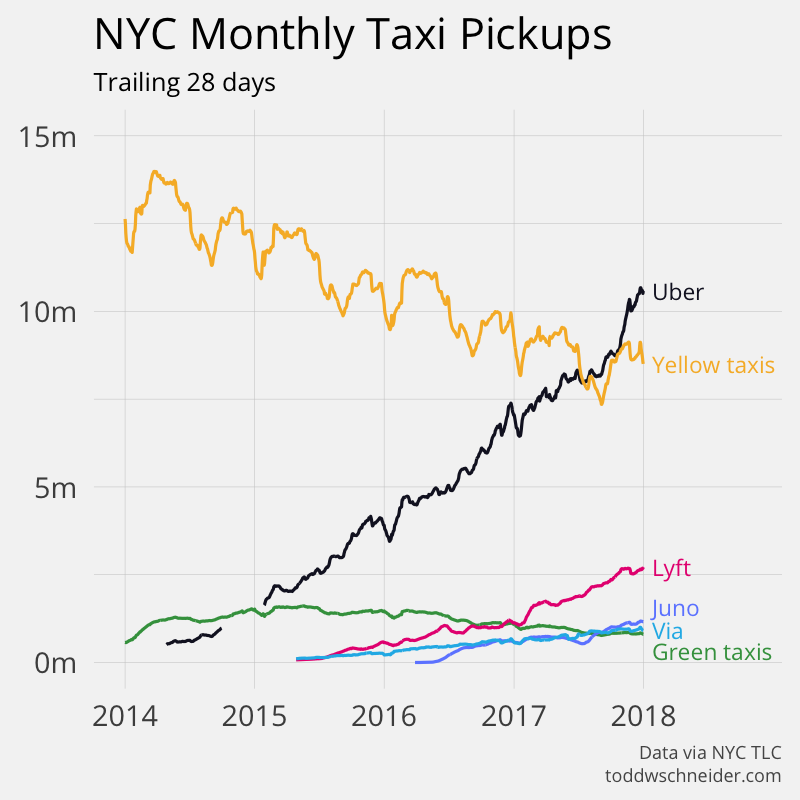
\includegraphics[width=4in]{figure/totals_by_car_type} \end{center}

As shown in the visulization above, which was generated by Todd W.
Schneider (Schneider, 2015), the number of New York City yellow taxi
trips has been consistently declining for about 4 years, and the numbers
of Uber and Lyft trips keep increasing. In 2017, for the first time, the
total number of monthly uber trips has exceeded the number of yellow
taxi trips.

Studies that show how competitive Uber and Lyft are have been done. In
2017, Uber and Lyft vehicles outnumbered NYC yellow cabs by 4 to 1.
(Sugar, 2017) Even though Yellow cab is still an icon of New York City,
passengers nowadays tend to choose the more convenient options,
ride-hailing apps.(Hu, 2017)

As reported in a jounal from Forbes Tech, data scientists from the
University of Cambridge in the UK and the University of Namur in Belgium
found that yellow taxi rides are on average \$1.4 cheaper than Uber X.
Moreover, uber appears more expensive for trips that are cheaper than
\$35, and less expensive than yellow taxi ride for trips that are more
expensive than \$35. Therefore, for short trips, taking a taxi is more
affordable. (Guerrini, 2015)

Apps, such as Openstreetcab, that compares the price of Uber and taxi
trips are designed to help customers to compare the fares of different
transportations. (``OpenStreetCab,'' 2015)

\section{Contribution}\label{contribution}

\subsection{\texorpdfstring{`nyctaxi'
Package}{nyctaxi Package}}\label{nyctaxi-package}

\texttt{nyctaxi} is an R package that help users to easily get access to
New York City Taxi, Uber and Lyft trip data through Extract, Transform,
and Load functions (ETL). (B. S. Baumer, 2017) This package facilitates
ETL to deal with medium data that are too big to store in memory on a
laptop. Users are given the option to choose specific years and months
as the input parameters of the three ETL functions, and a connection to
a populated SQL database will be returned as the output. Users do not
need to learn SQL queries, since all user interaction is in R.
\begin{Shaded}
\begin{Highlighting}[]
\KeywordTok{library}\NormalTok{(webshot)}
\end{Highlighting}
\end{Shaded}
\begin{verbatim}
Warning: package 'webshot' was built under R version 3.4.3
\end{verbatim}
\begin{Shaded}
\begin{Highlighting}[]
\KeywordTok{webshot}\NormalTok{(}\StringTok{"https://github.com/beanumber/nyctaxi"}\NormalTok{, }\StringTok{"r-nyctaxi.png"}\NormalTok{)}
\end{Highlighting}
\end{Shaded}
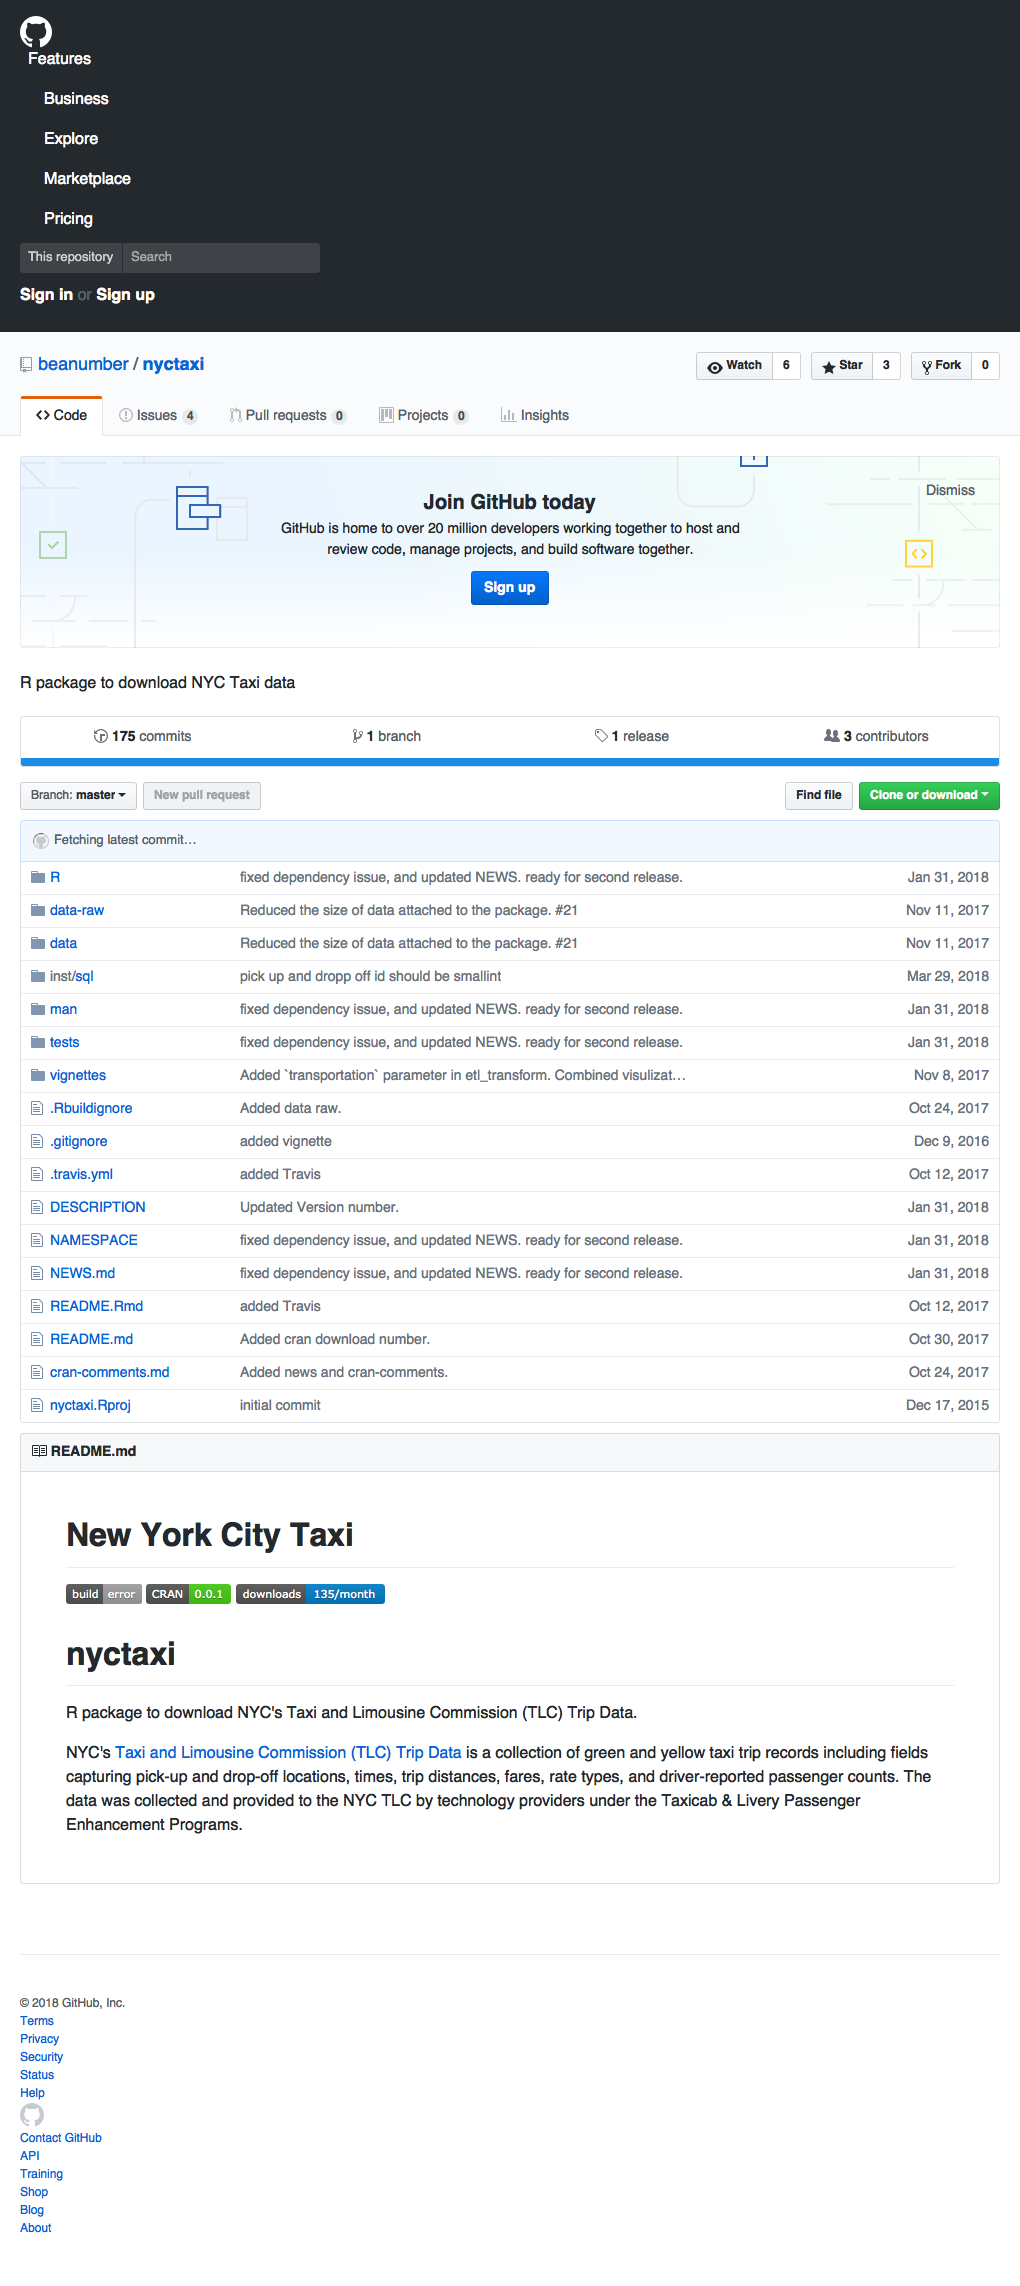
\includegraphics{thesis_files/figure-latex/unnamed-chunk-3-1.png}

\subsection{Social Impact of NYC Taxi}\label{social-impact-of-nyc-taxi}

NYC Taxi drivers wants to make the most profit. Taxi passengers want the
cheapest and most convenient way of transportantion. Since Uber and Lyft
launched their services in New York City, many consumers started to
demand the cheaper e-hail services.(Sugar, 2017) TLC wants to protect
both taxi drivers and passengers, and it creates policies to make NYC
taxi more accessible to consumers who really need this service. In these
sections, we analyze what each party wants and try to find a way for
them to be achieve their goals.

\subsection{Reproducible Research}\label{reproducible-research}

Reproducible research and open source are two main emphasis of my honors
project. As scholars place more emphasis on the reproducibility of
research studies, it is essential for me to make my data and code openly
available for people to redo the analysis.

\texttt{Knitr} and Github are used in my project to make my study
reproducible, ranging from the initial source to raw data to the package
I wrote to utlize the raw data to the statistical data analysis. I used
an R package called \texttt{thesisdown} to layout the basic structure of
my paper, this tool allows students to create reproducible and dynamic
techinical report in R Markdown. It also allows users to embed R code
and interactive applicationis, and output into PDF, Word, ePub, or
gitbook doocuments. \texttt{thesisdown} helps users to efficiently put
together any paper with similar format.

Github is used to store the scripts for \texttt{nyctaxi} and this
thesis. \texttt{nyctaxi} is available on CRAN for people to download and
install (B. Baumer, Li, \& Le, 2017), and the source code for data
analysis in this thesis is available under the Github account of the
author so that scholars can easily access the information that thery are
interested in. In terms of tables, figures, and anything included in the
Appendix attached to this thesis, scripts that are used to generate them
are included in the Github repository.

\chapter{Data and nyctaxi Package}\label{chapter2}

\section{Data and Storage}\label{data-and-storage}

The \texttt{nyctaxi} R package allows users to download, clean, and load
data into SQL databasses. There are four types of data that are
available for users to get access to, and they are trip level yellow
taxi data from 2009 to the most recent month, trip level green taxi data
from August 2013 to the most recent month, uber pick-up data from April
to September 2014 and from Janaury to June 2015, and weekly-aggregated
lyft trip data from 2016 to the most recent week. (B. Baumer et al.,
2017)

\subsection{Yellow Taxi}\label{yellow-taxi-1}

The total size of all yellow taxi trip data \texttt{csv} files (from Jan
2010 to Dec 2016) is 191.38 GB, and NYC yellow taxi trip data from Jan
2009 to the most recent month can be found on the NYC Taxi \& Limousine
Commission (TLC) website. (``TLC Trip Record Data,'' 2009a) The data
were collected and provided to the NYC TLC by technology providers
authorized under the Taxicab \& Livery Passenger Enhancement Programs
(TPEP/LPEP).

The yellow taxi trip records include the following fields: pick-up and
drop-off dates/times, pick-up and drop-off locations, trip distances,
itemized fares, rate types, payment types, and driver-reported passenger
counts.

\subsection{Green Taxi}\label{green-taxi-1}

The total size of green taxi trip data \texttt{csv} files (from Aug 2013
to Dec 2016) is 7.8 GB, and green taxi trip data from Aug 2013 to the
most recent month can be downloaded from NYC Taxi \& Limousine
Commission (TLC). (``TLC Trip Record Data,'' 2009a) Green taxi trip
records include the same variables as yellow taxi trip records do.

\subsection{TLC Summary Report}\label{tlc-summary-report}

The New York City TLC publishes summary reports that include aggregate
statistics about taxi, Uber, and Lyft usage. These are in addition to
the trip-level data; although the summary reports contain much less
detail, they're updated more frequently, which provides a more current
glimpse into the state of the cutthroat NYC taxi market. (``TLC
Aggregated Reports,'' 2009)

In addition, the trip level NYC Uber data only covers two periods, from
April to September 2014 and from January to June 2015. However, the
summary reports cover weekly-aggreagated data from 2015 to the most
recent week.

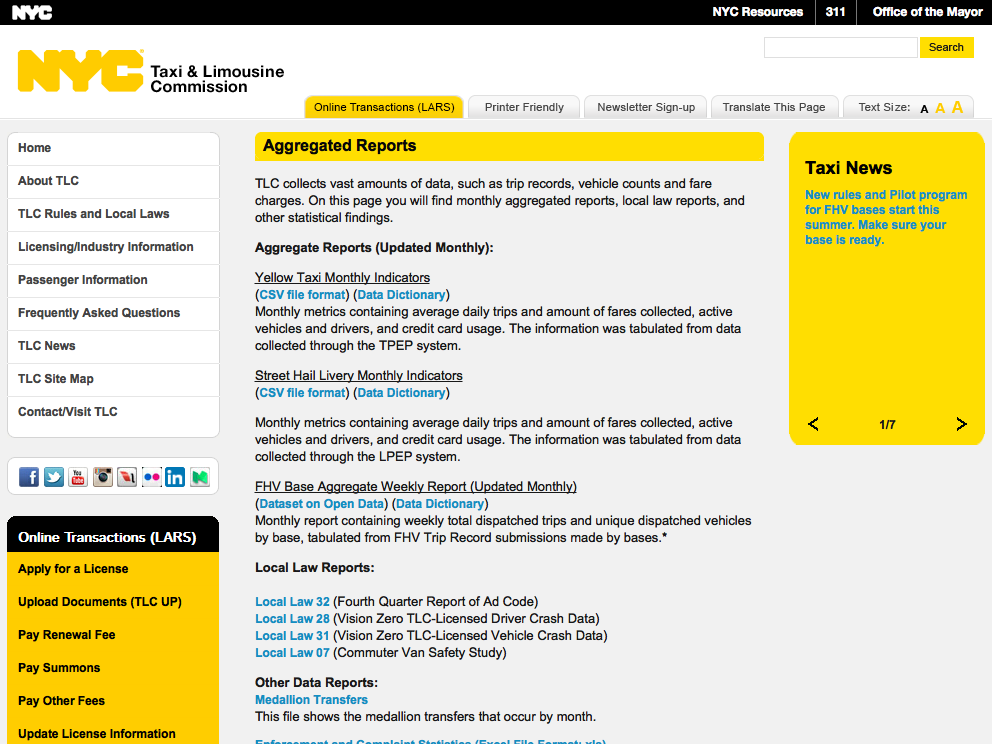
\includegraphics{thesis_files/figure-latex/unnamed-chunk-5-1.png}
\begin{center}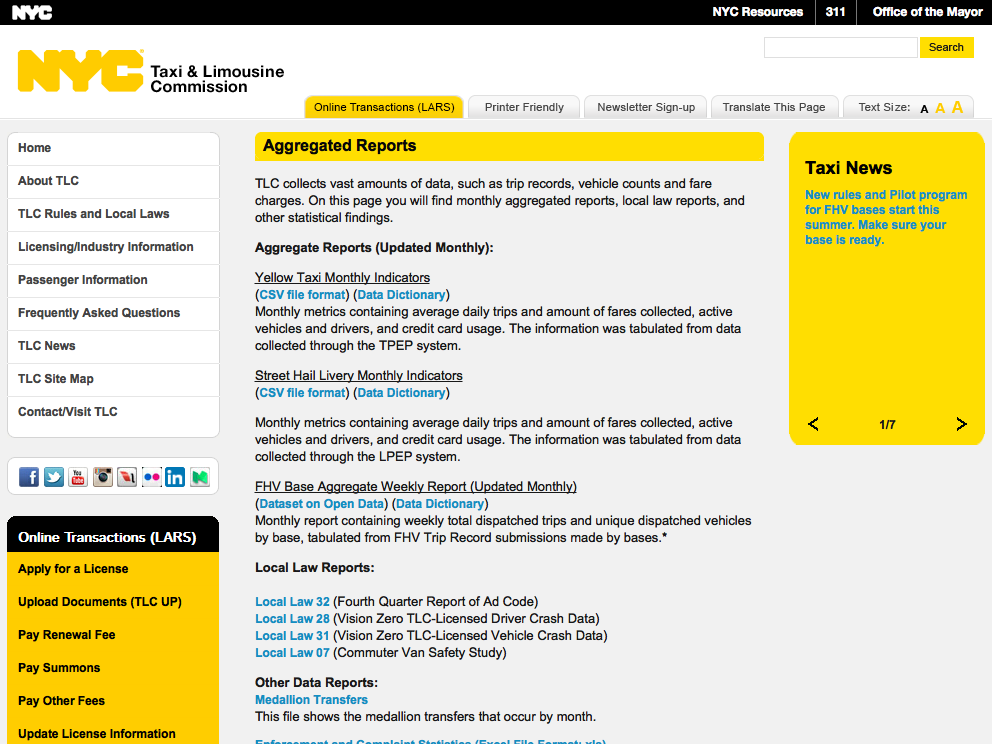
\includegraphics[width=4.96in]{figure/a-report} \end{center}

The data can be accessed by using the following commands: * Yellow taxi
data
\begin{Shaded}
\begin{Highlighting}[]
\KeywordTok{download.file}\NormalTok{(}\StringTok{"http://www.nyc.gov/html/tlc/downloads/csv/data_reports_monthly_indicators_yellow.csv"}\NormalTok{, }
    \DataTypeTok{destfile =} \StringTok{"~/Desktop/yellow_monthly_data.csv"}\NormalTok{)}
\end{Highlighting}
\end{Shaded}
*Uber and Lyft data
\begin{Shaded}
\begin{Highlighting}[]
\KeywordTok{download.file}\NormalTok{(}\StringTok{"http://data.cityofnewyork.us/api/views/2v9c-2k7f/rows.csv?accessType=DOWNLOAD"}\NormalTok{, }
    \DataTypeTok{destfile =} \StringTok{"~/Desktop/fhv_weekly_data.csv"}\NormalTok{)}
\end{Highlighting}
\end{Shaded}
\subsection{Uber}\label{uber-1}

The total size of Uber pick-up data (from Apr to Sep 2014 and from Jan
to June 2015) is 4.3 MB, and thanks to FiveThirtyEight who obtained the
data from NYC TLC by submitting a Freedom of Information Law request on
July 20, 2015, these data are now open to public. (``TLC Trip Record
Data,'' 2009b)

The 2014 Uber data contains four variables: Date/Time (the date and time
of the Uber pick-up), Lat (the latitude of the Uber pick-up), Lon (the
longitude of the Uber pick-up), and Base (the TLC base company code
affiliated with the Uber pickup).

The 2015 Uber data contains four variables: Dispatching\_base\_num (the
TLC base company code of the base that dispatched the Uber),
Pickup\_date (the date of the Uber pick-up), Affiliated\_base\_num (the
TLC base company code affiliated with the Uber pickup), and locationID
(the pick-up location ID affiliated with the Uber pickup).

NYC Open Data also provides weekly-aggreagated Uber pick-up data from
2015 to the most recent month. (``Uber Trips NYC 2016,'' 2015)

\subsection{Lyft}\label{lyft-1}

The total size of weekly-aggregated Lyft trip data (from Jan 2015 to Dec
2016) is 914.9 MB, and these data are open to public and
weekly-aggregated Lyft data from 2015 to the most recent week can be
found on NYC OpenData website. (``LYFT Data,'' 2015)

\subsection{Data Storage}\label{data-storage}

The total size of all \texttt{csv} files of the four services is about
200 GB, and a laptop usually has memory less than or equal to 8 GB.
Limited memory constrains the amount of data that can be loaded by a
personal computer at one time. When users load data into R environment,
R keeps them in memory; when the amount of data loaded into R
environment gets close to the limit of a computer's memory, R becomes
unresponsive or force quit the current session. Therefore, better ways
to work with data that takes more space than 8 GB is needed. According
to Weijia Zhang (2016), comparing to RAM, hard disk is often used to
store medium-sized data, because it is affordable and are designed for
storing large items permanently. However, retrieving data from hard
drives usually takes about 1,000,000 times more time.

\section{ETL nyctaxi Package}\label{etl-nyctaxi-package}

\texttt{etl} is the parent package of \texttt{nyctax}. \texttt{etl}
provides a framework that allows R users to work with medium data
without any knowledge in SQL database. Users can run SQL queries by
using \texttt{dplyr} commands in R and choose to only return the final
result, which could be a summary table, from SQL database into R
Environment in order to aovid R from crashing. The user interaction
takes place solely within R.

\texttt{etl} framework has three operations -Extract, Transfer, and
Load- which bring real-time data into local or remote SQL databases.
Users can specify which type of SQL database they prefer to connect to.
\texttt{etl}-dependent packages, such as \texttt{nyctaxi}, make medium
data more accessible to a wider audience. (B. Baumer et al., 2014)

\texttt{nyctaxi} was initially designed to work with New York City taxi
data, but later on Uber and Lyft data were added and the ETL functions
are modified to be specialized in working with these data. This package
compiled three major sources of hail service in New York City so that it
is convenient for users to compare and contrast the performance of these
three services. (B. Baumer et al., 2017)

This package inherits functions from many packages: \texttt{etl},
\texttt{dplyr}, \texttt{DBI}, \texttt{rlang}, and \texttt{stringr}.

Since SQL databases are good tools for medium data analysis, ETL
functions build connection to a SQL database at the back end and convert
R code automatically into SQL queries and send them to the SQL database
to get data tables containing data of each hail service. Thus, users do
not need to have any knowledge of SQL queries and they can draw in any
subsets of the data from the SQL database in R.

In general, \texttt{etl\_extract.etl\_nyctaxi()} function download data
of the four types of hail service data (yellow taxi, green taxi, uber,
and lyft) from the corresponding sources. transform.nyctaxi uses
different techniques to clean all four types of data to get then ready
for the next step. \texttt{etl\_load.etl\_nyctaxi()} loads the data user
selected to a SQL database.

The Comprehensive R Archive Network (CRAN) is a collection of sites that
carry identical material, consisting of the R distributions, the
contributed extensions, documentation for R, and binaries. (Studio,
n.d.) \texttt{nyctaxi} R package lives on CRAN, and it can be installed
with the \texttt{install.packages()} function in R.
\begin{Shaded}
\begin{Highlighting}[]
\CommentTok{# install the package}
\KeywordTok{install.packages}\NormalTok{(}\StringTok{"nyctaxi"}\NormalTok{)}
\end{Highlighting}
\end{Shaded}
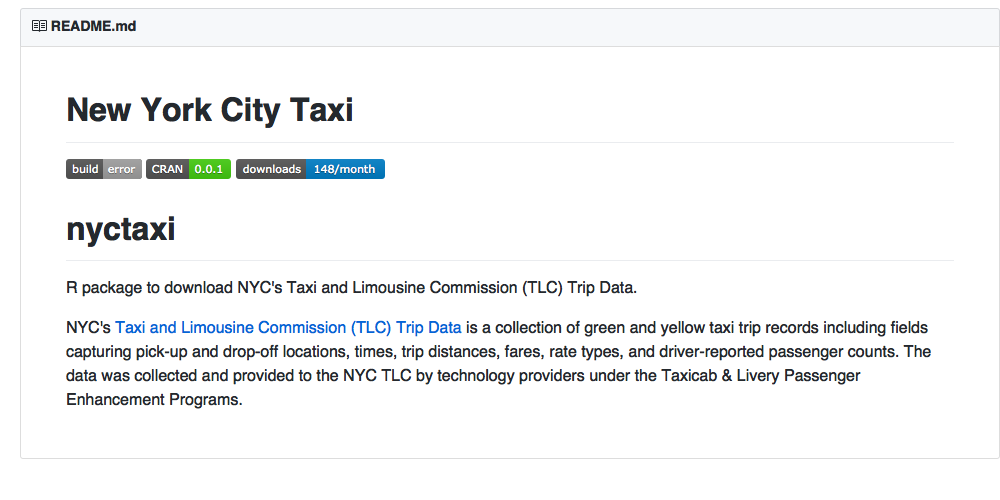
\includegraphics{thesis_files/figure-latex/unnamed-chunk-10-1.png}
\begin{center}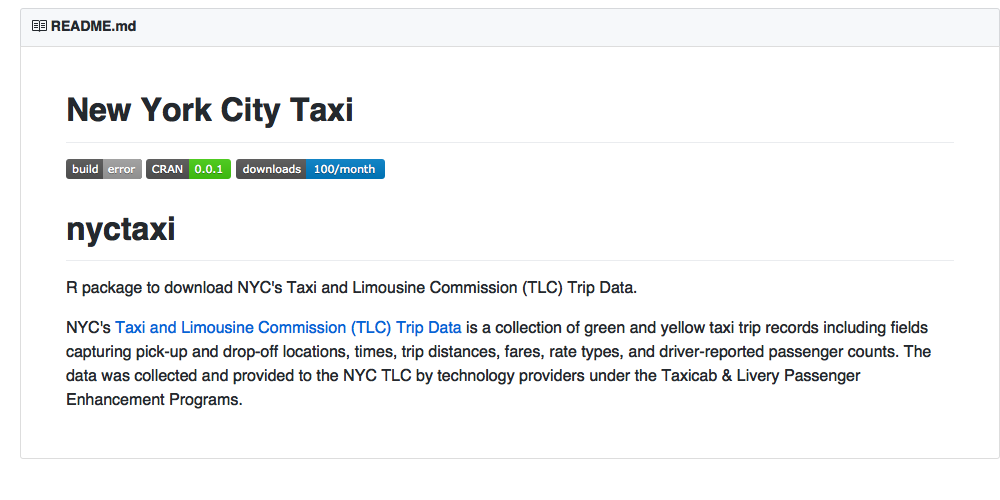
\includegraphics[width=5in]{figure/nyctaxi-page} \end{center}
\begin{verbatim}
Warning: package 'RMySQL' was built under R version 3.4.3
\end{verbatim}
\begin{verbatim}
Warning: package 'DBI' was built under R version 3.4.3
\end{verbatim}
Users need to create an etl object in order to apply the etl operations
to it, and only the name of the SQL database, working directory, and
type of SQL database need to be specified during initialization. If the
type of SQL database is not specified, a local RSQLite database will be
generated as default.
\begin{Shaded}
\begin{Highlighting}[]
\CommentTok{# initializing an etl object}
\NormalTok{db <-}\StringTok{ }\KeywordTok{src_mysql}\NormalTok{(}\StringTok{"nyctaxi"}\NormalTok{, }\DataTypeTok{user =} \StringTok{"urname"}\NormalTok{, }\DataTypeTok{host =} \StringTok{"host"}\NormalTok{, }
    \DataTypeTok{password =} \StringTok{"pw"}\NormalTok{)}
\NormalTok{taxi <-}\StringTok{ }\KeywordTok{etl}\NormalTok{(}\StringTok{"nyctaxi"}\NormalTok{, }\DataTypeTok{dir =} \StringTok{"~/Desktop/nyctaxi"}\NormalTok{, db)}
\end{Highlighting}
\end{Shaded}
In the example above, a folder called nyctaxi is created on the desktop
and a connection to a MySQL database is generated. In the procession of
initialization, a local folder contains two subfolders, \texttt{raw} and
\texttt{load}, are also created under the directory the user specifies.
\texttt{raw} folder stores data downloaded from online open sources, and
\texttt{load} folder stores cleaned CSV data files that are ready to be
loaded into SQL database. The ETL framework keeps data directly scraped
from online data sources in their original forms. In this way, the
original data is always available to users in case data corruption
happens in later stages.

After an etl object is created (nyctaxi is the etl object in this case),
four parameters are needed to specify the data that users want: (1)
\texttt{obj}: an etl object; (2) \texttt{years}: a numeric vector giving
the years, and the default is the most recent year; (3) \texttt{months}:
a numeric vector giving the months, and the default is \texttt{1:12};
(4) \texttt{type}: a character variable giving the type of data the user
wants to download. There are four types: yellow, green, uber, and lyft.
The default is yellow.

\subsection{Taxi zone shapefile attached to nyctaxi R
package}\label{taxi-zone-shapefile-attached-to-nyctaxi-r-package}

Two datasets are attached to \texttt{nyctaxi}. The first one is called
\texttt{taxi\_zone\_lookup}, and this dataset contains information, such
as taxi zone location IDs, location names, and corresponding boroughs
for each ID. (``TLC Trip Record Data,'' 2009a) A shapefile containing
the boundaries for the taxi zones, \texttt{taxi\_zones}, is also
included in the package for users to do spatial analysis. Visulizations
similar to one shown below can be generated with the shapefile.
\begin{verbatim}
Warning: package 'sp' was built under R version 3.4.3
\end{verbatim}
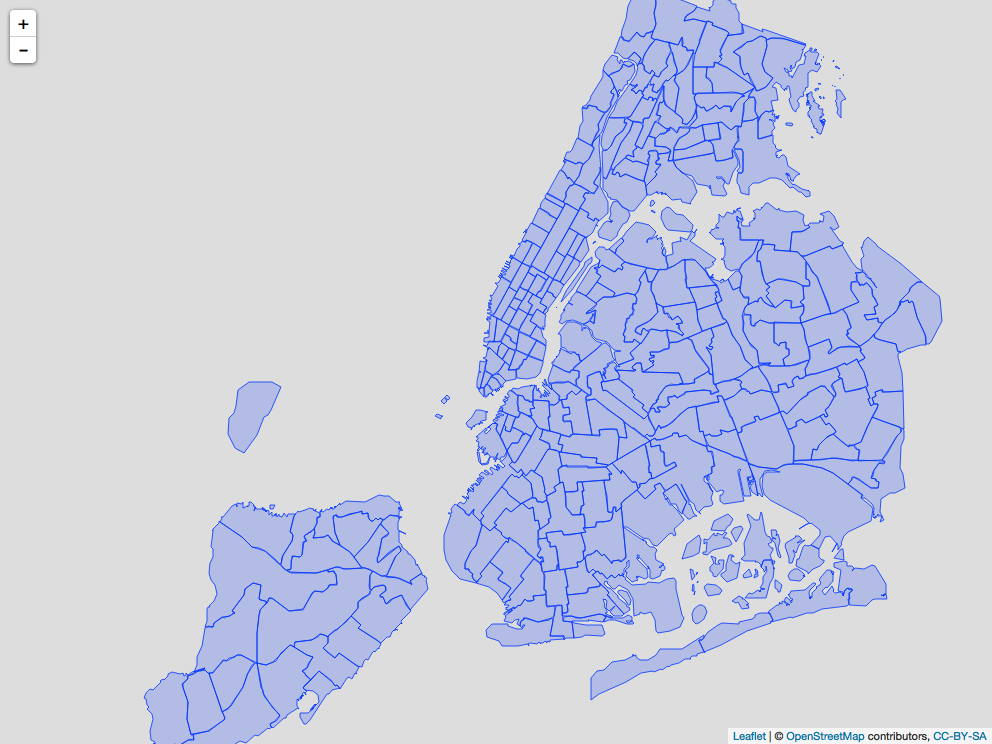
\includegraphics{thesis_files/figure-latex/unnamed-chunk-14-1.png}
\begin{figure}

{\centering 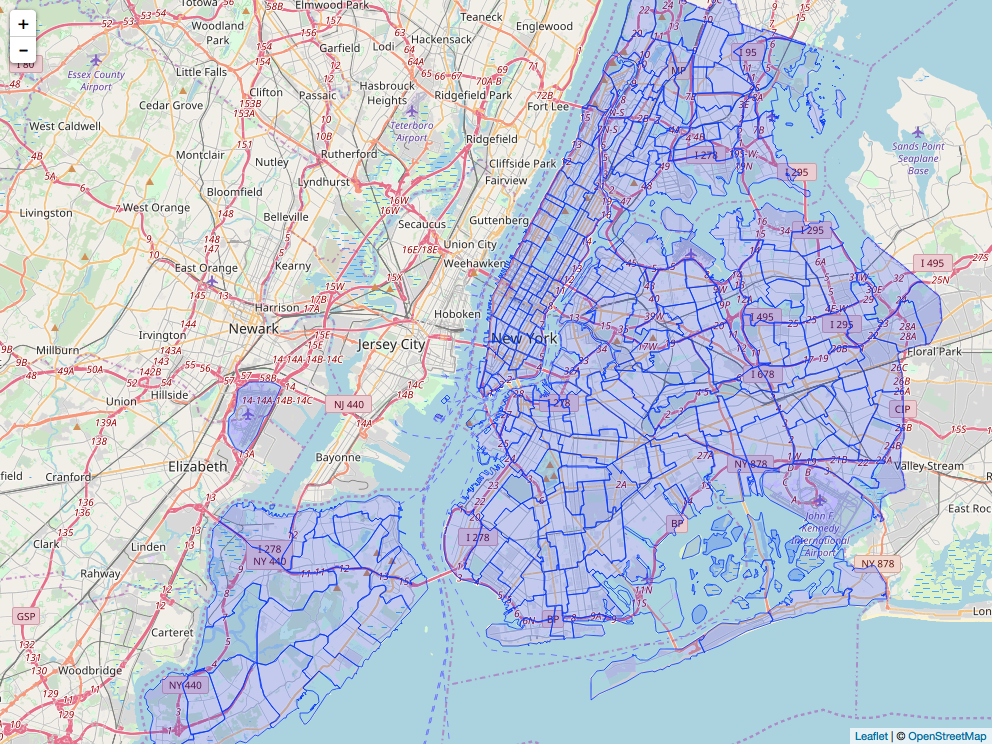
\includegraphics[width=4.96in]{figure/zonemap} 

}

\caption{NYC Taxi Zone Map}\label{fig:map}
\end{figure}
\section{Extract-Transform-Load}\label{extract-transform-load}

\subsection{Extract}\label{extract}

\texttt{etl\_extract.nyctaxi} allows users to download New York City
yellow taxi, green taxi, Uber, and Lyft data from the corresponding data
sources. It takes the \texttt{years}, \texttt{months}, and \texttt{type}
parameters and download the New York City taxi data specified by users.
New York City Yellow and Green Taxi data are updated on NYC Taxi \&
Limousine Commission (TLC) website on a monthly basis.

Uber trip record data is static and small, so we decided to only give
users the options to either download all data from April to Sepetember,
2014 or download all Uber trip records from Janaury to June, 2015 at
onc. Users do not have the lesuire to download Uber data from a specific
month.

Lyft data is updated on NYC Open Data webiste on a weekly basis. Since
the weekly-aggregated data is tiny and only data later then 2014 is
available, we decided to only allow users to download Lyft data by year.

The default \texttt{years} is the current year, and the default
\texttt{months} are the all twelve months. The default type of
transportation is \texttt{yellow}. When an invalid month is entered,
warning message will suggest users to reconsider their choice and select
a new set of month.

\subsection{Transform}\label{transform}

\texttt{etl\_transform.nyctaxi} allows users to transform New York City
yellow taxi, green taxi, Uber, and Lyft data into cleaned formats, and
it utlizes different data cleaning techiniques when it transforms data
for each transportation type. In general, it cleans the data and creates
a new \texttt{csv} file in the \texttt{load} directory to store the
cleaned data. It helps us to retain and protect raw data from being
mondified or destroyed. Users are allows to specify the month of
interest in order to only transform the data that they are interested
in. This functionality helps people to be more efficient with their use
of time.

By default, it takes the current year Yellow taxi trip records data
files, and save copies of them in the \texttt{load} diectory. It skips
the cleaning step, because the raw Yellow Taxi data downloaded from TLC
is already in a desired format with all variables correctly labelled.

There are a few main transformations that are done by this fucntion:

\subsubsection{Green Taxi -- Extra Blank Row and
Column}\label{green-taxi-extra-blank-row-and-column}

Green Taxi monthly data from August 2013 to the most recent month
besides 2015 all have a blank second row in the \texttt{csv} files.
Similar to this problem, Green Taxi data from 2013, 2014, and 2015 all
have an extra blank columns attanched to the right-most column. These
blank row and solumn causes problems in the later stage when users want
to load data into SQL database. In order to get Green Taxi data ready
for the \texttt{load} phase, we used \texttt{system()} to invoke the OS
command specified to remove the blank rows and columns.

\subsubsection{Uber Data -- Reconciling Inconsistent
Filenames}\label{uber-data-reconciling-inconsistent-filenames}

Uber only released over 4.5 million data records from April to Sepetmber
2014 and 14.3 million records from Janaury to June 2015. Information of
different sets of variables are released for 2014 and 2015, and
variables have different naming convention. When users want to download
data from both years, variables are renamed so that data from both years
can be cosolidated into one big dataset with consistent variable names.

\subsubsection{Uber Data -- Reconciling Inconsistent Data
Formats}\label{uber-data-reconciling-inconsistent-data-formats}

The data type of \texttt{Date/Time} variable in Uber datasets is
originally encoded as \texttt{character}. In order to enable it to be
recognized as \texttt{timestamp} by R, we use \texttt{ymd\_hms} in
\texttt{lubridate} to transform date time to POSIXct objects.

\subsubsection{Optimizing I/O Process}\label{optimizing-io-process}

h p://scholarworks.smith.edu/theses/1871 Zhang, Weijia, ``Improving
access to open-source data about the NYC bike sharing system (Citi
Bike)'' (2017). eses, Dissertations, and Projects. 1871.

Meking the file inout and output processes more efficient is an
important pasrt of \texttt{etl\_transform}. According to Zhang's (2017)
study, \texttt{data.table} only takes half of the time to read from and
write into datasets comparing to \texttt{readr}. Therefore,
\texttt{etl\_transform} uses \texttt{fread()} and \texttt{fwrite()} from
\texttt{data.table} instead of \texttt{read\_csv} or \texttt{write\_csv}
from \texttt{readr} to reduce the data processing time.

\subsection{Load}\label{load}

\texttt{etl\_load.nyctaxi} allows users to load New York City yellow
taxi, green taxi, Uber, and Lyft data into different data tables in a
SQL database. It populates a SQL database with data cleaned by
\texttt{etl\_transform}. In order to reduce the data processing
complexity, \texttt{init.mysql()} is written under \texttt{nyctaxi} to
help users to set up five basic table structures for MySQL database.

\subsection{SQL Database
Initialization}\label{sql-database-initialization}

\texttt{init.mysql()} helps users to set up five basic table structures
for MySQL database. \texttt{yellow\_old} is created for Yellow Taxi data
that are prior to August 2016, and \texttt{yellow} is created for data
later than July 2016. \texttt{green}, \texttt{uber}, and \texttt{lyft}
are also initiated for the three transportations.

\texttt{etl\_init()} can be run after a database connection is built to
process to process \texttt{init.mysql()} to initialize a MySQL database,
and default columns with the correct variable names and typed defined
will be automatically generated.
\begin{Shaded}
\begin{Highlighting}[]
\NormalTok{taxi }\OperatorTok\StringTok{ }\KeywordTok{etl_init}\NormalTok{()}
\end{Highlighting}
\end{Shaded}
In order to increase the query speed at the data analysis stage,
\texttt{KEY}s are created for multiple variables for each
transportation. Since there is no variable containing unique value for
each observation, no primary variable is needed. Using \texttt{KEY} in
data analysis query can spped up the query process.

Due to the large size of Yellow Taxi datasets, \texttt{yellow\_old} and
\texttt{yellow} are partitioned into subgroups by \texttt{year}. When we
need to run query on data from a specific year, having partitions allows
MySQL to directly find the data specified without filtering on every
single row. It speeds up the query process. A \texttt{VIEW} called
\texttt{yellow\_old\_sum} is also created to generate a summary table
for the number of Yellow Taxi trips in each month.

\section{New Yoek City Street-hail and E-hail Services
Summary}\label{new-yoek-city-street-hail-and-e-hail-services-summary}

Below is a summary of data that are available to users from 2014 to
2016.The Uber data used to create the summary below is the trip-level
data from Uber TLC FOIL Response.
\begin{figure}

{\centering 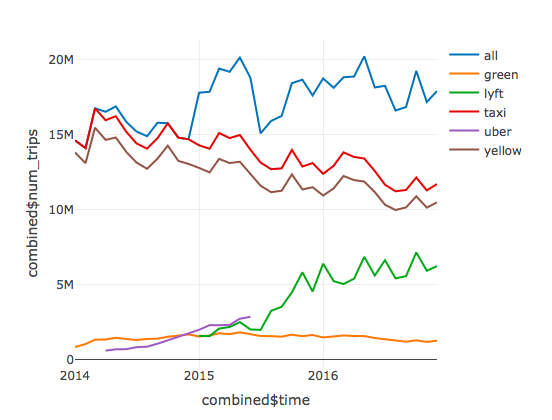
\includegraphics[width=2.76in]{figure/Num_trips_summary} 

}

\caption{Summary of Number of trips Made by 4 Types of Transportations between 2014 and 2016 in NYC, }\label{fig:num-trips-summary}
\end{figure}
A similar summary of data can also be created by combining monthly
yellow taxi data from TLC Aggregated Reports and weekly Uber and Lyft
data from NYC OpenData. These data can be downloaded by running the code
below:
\begin{itemize}
\tightlist
\item
  Yellow taxi monthly data
\end{itemize}
\begin{Shaded}
\begin{Highlighting}[]
\KeywordTok{download.file}\NormalTok{(}\StringTok{"http://www.nyc.gov/html/tlc/downloads/csv/data_reports_monthly_indicators_yellow.csv"}\NormalTok{, }
    \DataTypeTok{destfile =} \StringTok{"~/Desktop/yellow_monthly_data.csv"}\NormalTok{)}
\end{Highlighting}
\end{Shaded}
\begin{itemize}
\tightlist
\item
  Uber weekly data
\end{itemize}
\begin{Shaded}
\begin{Highlighting}[]
\KeywordTok{download.file}\NormalTok{(}\StringTok{"https://data.cityofnewyork.us/resource/gt3n-7ri6.csv"}\NormalTok{, }
    \DataTypeTok{destfile =} \StringTok{"~/Desktop/uber_weekly_data.csv"}\NormalTok{)}
\end{Highlighting}
\end{Shaded}
\begin{itemize}
\tightlist
\item
  Lyft weekly data
\end{itemize}
\begin{Shaded}
\begin{Highlighting}[]
\KeywordTok{download.file}\NormalTok{(}\StringTok{"https://data.cityofnewyork.us/resource/juxc-sutg.csv"}\NormalTok{, }
    \DataTypeTok{destfile =} \StringTok{"~/Desktop/lyft_weekly_data.csv"}\NormalTok{)}
\end{Highlighting}
\end{Shaded}
\section{Source Code}\label{source-code}

\subsection{ETL Extract}\label{etl-extract}
\begin{verbatim}
opts_chunk$set(tidy.opts=list(width.cutoff=60))

etl_extract.etl_nyctaxi <- 
  function(obj, 
years = as.numeric(format(Sys.Date(),'%Y')), 
                                    months = 1:12, 
                                    type  = "yellow",...) {
  #TAXI YELLOW-------------------------
  taxi_yellow <- function(obj, years, months,...) {
    message("Extracting raw yellow taxi data...")
    remote <- etl::valid_year_month(years, months, 
    begin = "2009-01-01") %>%
      mutate_(src = 
  ~file.path("https://s3.amazonaws.com/nyc-tlc/trip+data", 
                               paste0("yellow", "_tripdata_", year, "-",
                      stringr::str_pad(month, 2, "left", "0"), ".csv"))) 
    tryCatch(expr = etl::smart_download(obj, remote$src, ...),
             error = function(e){warning(e)}, 
             finally = warning("Only the following data are availabel on
                                TLC: Yellow taxi data: 2009 Jan - 
                               last month"))} 
  #TAXI GREEN----------------------
  taxi_green <- function(obj, years, months,...) {
    message("Extracting raw green taxi data...")
    remote <- etl::valid_year_month(years, months, begin = "2013-08-01") %>%
      mutate_(src = 
                ~file.path("https://s3.amazonaws.com/nyc-tlc/trip+data", 
                               paste0("green", "_tripdata_", year, "-",
                          stringr::str_pad(month, 2, "left", "0"), ".csv")))
    tryCatch(expr = etl::smart_download(obj, remote$src, ...),
             error = function(e){warning(e)}, 
             finally = warning("Only the following data are availabel on TLC:
                               Green taxi data: 2013 Aug - last month"))} 
  #UBER--------------------------------
  uber <- function(obj, years, months,...) {
    message("Extracting raw uber data...")
    raw_month_2014 <- etl::valid_year_month(years = 2014, months = 4:9)
    raw_month_2015 <- etl::valid_year_month(years = 2015, months = 1:6)
    raw_month <- bind_rows(raw_month_2014, raw_month_2015)
    path = "https://raw.githubusercontent.com/
    fivethirtyeight/uber-tlc-foil-response/master/uber-trip-data"
    remote <- etl::valid_year_month(years, months)
    remote_small <- intersect(raw_month, remote)
    if (2015 %in% remote_small$year && !(2014 %in% remote_small$year)){
      #download 2015 data
      message("Downloading Uber 2015 data...")
      etl::smart_download(obj, "https://github.com/fivethirtyeight/
                          uber-tlc-foil-response/raw/master/
                    uber-trip-data/uber-raw-data-janjune-15.csv.zip",...)}
    else if (2015 %in% remote_small$year && 2014 %in% remote_small$year) {
      #download 2015 data
      message("Downloading Uber 2015 data...")
      etl::smart_download(obj, "https://github.com/fivethirtyeight/
                        uber-tlc-foil-response/raw/master/uber-trip-data
                          /uber-raw-data-janjune-15.csv.zip",...)
      #download 2014 data
      small <- remote_small %>%
        filter_(~year == 2014) %>%
        mutate_(month_abb = ~tolower(month.abb[month]),
                src = ~file.path(path,
                paste0("uber-raw-data-",month_abb,
                substr(year,3,4),".csv")))
      message("Downloading Uber 2014 data...")
      etl::smart_download(obj, small$src,...) 
    } else if (2014 %in% remote_small$year && 
    !(2015 %in% remote_small$year)) {
      message("Downloading Uber 2014 data...")
      #file paths
      small <- remote_small %>%
        mutate_(month_abb = 
                  ~tolower(month.abb[month]),
                src = ~file.path(path,
                paste0("uber-raw-data-",month_abb,
                substr(year,3,4),".csv")))
      etl::smart_download(obj, small$src,...)}
    else {warning("The Uber data you requested are 
                  not currently available. Only data
                  from 2014/04-2014/09 and 2015/01-
                  2015/06 are available...")}
    } 
  #LYFT----------------------------------
  lyft <- function(obj, years, months,...){
    message("Extracting raw lyft data...")
    #check if the week is valid
    valid_months <- etl::valid_year_month(years, months,
    begin = "2015-01-01")
    base_url = "https://data.cityofnewyork.us/
    resource/edp9-qgv4.csv"
    valid_months <- valid_months %>%
      mutate_(new_filenames = 
                ~paste0("lyft-", year, ".csv")) %>%
      mutate_(drop = TRUE)
    #only keep one data set per year
    year <- valid_months[1,1]
    n <- nrow(valid_months)
    for (i in 2:n) {
      if(year == valid_months[i-1,1]) {
        valid_months[i,6] <- FALSE
        year <- valid_months[i+1,1]
      } else {
        valid_months[i,6] <- TRUE
        year <- valid_months[i+1,1]}
      }
    row_to_keep = valid_months$drop
    valid_months <- valid_months[row_to_keep,]
    
    #download lyft files, try two different methods
    first_try<-tryCatch(
      download_nyc_data(obj, base_url, valid_months$year, 
      n = 50000, names = valid_months$new_filenames),
      error = function(e){warning(e)},
      finally = 'method = "libcurl" fails')
  }
  
  if (type == "yellow"){taxi_yellow(obj, years, months,...)} 
  else if (type == "green"){taxi_green(obj, years, months,...)}
  else if (type == "uber"){uber(obj, years, months,...)}
  else if (type == "lyft"){lyft(obj, years, months,...)}
  else {message("The type you chose does not exit...")}
  
  invisible(obj)
}
\end{verbatim}
\subsection{ETL Transform}\label{etl-transform}
\begin{verbatim}
opts_chunk$set(tidy.opts=list(width.cutoff=60))
etl_transform.etl_nyctaxi <- function(obj, 
                          years = as.numeric(format(Sys.Date(),'%Y')), 
                          months = 1:12, 
                          type  = "yellow",...) {
  #TAXI YELLOW-----------------------------
  taxi_yellow <- function(obj, years, months) {
    message("Transforming yellow taxi data from raw to 
            load directory...")
    #create a df of file path of the files that the user wants to transform
    remote <- etl::valid_year_month(years, months, 
    begin = "2009-01-01") %>%
      mutate_(src = ~file.path(attr(obj, "raw_dir"), 
      paste0("yellow", "_tripdata_", year, "-",
      stringr::str_pad(month, 2, "left", "0"), ".csv"))) 
    #create a df of file path of the files that are in the raw directory
    src <- list.files(attr(obj, "raw_dir"), "yellow", full.names = TRUE)
    src_small <- intersect(src, remote$src)
    #Move the files
    in_raw <- basename(src_small)
    in_load <- basename(list.files(attr(obj, "load_dir"), "yellow", 
    full.names = TRUE))
    file_remian <- setdiff(in_raw,in_load)
    file.copy(file.path(attr(obj, "raw_dir"),file_remian),
              file.path(attr(obj, "load_dir"),file_remian) )}
  #TAXI GREEN-----------------------------
  taxi_green <- function(obj, years, months) {
    message("Transforming green taxi data from raw 
            to load directory...")
    #create a df of file path of the files that the user wants to transform
    remote <- etl::valid_year_month(years, months, 
    begin = "2013-08-01") %>%
      mutate_(src = ~file.path(attr(obj, "raw_dir"), 
      paste0("green", "_tripdata_", year, "-",
      stringr::str_pad(month, 2, "left", "0"), ".csv"))) 
    #create a df of file path of the files that are in the raw directory
    src <- list.files(attr(obj, "raw_dir"), "green", full.names = TRUE)
    src_small <- intersect(src, remote$src)
    #Clean the green taxi data files
    #get rid of 2nd blank row
    if (length(src_small) == 0){
      message("The files you requested are not available 
              in the raw directory.")
    } else{
      #a list of the ones that have a 2nd blank row
      remote_green_1 <- remote %>% filter_(~year != 2015)
      src_small_green_1 <- intersect(src, remote_green_1$src)
      # check that the sys support command line, 
      #and then remove the blank 2nd row
      if(length(src_small_green_1) != 0) {
        if (.Platform$OS.type == "unix"){
          cmds_1 <- paste("sed -i -e '2d'", src_small_green_1)
          lapply(cmds_1, system)
        } else {
          message("Windows system does not 
          currently support removing the 2nd blank row
          in the green taxi datasets. This might affect 
          loading data into SQL...")}
        }else {
          "You did not request for any 
          green taxi data, or all the green
          taxi data you requested are cleaned."}
      #fix column number
      remote_green_2 <- remote %>%
        filter_(~year %in% c(2013, 2014, 2015)) %>%
        mutate_(keep = 
                  ~ifelse(year %in% c(2013,2014), 20,21),
                new_file = 
                  ~paste0("green_tripdata_", year, "_", 
                      stringr::str_pad(month, 2, "left", "0"),
                                   ".csv"))
      src_small_green_2 <- intersect(src, remote_green_2$src)
      src_small_green_2_df <- data.frame(src_small_green_2) 
      names(src_small_green_2_df) <- "src"
      src_small_green_2_df <- inner_join(src_small_green_2_df, 
      remote_green_2, by = "src")
      src_small_green_2_df <- src_small_green_2_df %>%
        mutate(cmds_2 = paste("cut -d, -f1-", keep," ",src, " > ",
        attr(obj, "raw_dir"),"/green_tripdata_", 
        year, "_", stringr::str_pad(month, 2, "left", "0"),".csv", 
        sep = ""))
      #remove the extra column
      if(length(src_small_green_2) != 0) {
        if (.Platform$OS.type == "unix"){
          lapply(src_small_green_2_df$cmds_2, system)} 
        else {
          message("Windows system does not currently 
          support removing the 2nd blank row 
          in the green taxi datasets. This might 
          affect loading data into SQL...")}
        }else {
          "All the green taxi data you
          requested are in cleaned formats."}
      #Find the files paths of the files that need to be transformed
      file.rename(file.path(dirname(src_small_green_2_df$src),
                            src_small_green_2_df$new_file), 
                  file.path(attr(obj, "load_dir"),
                  basename(src_small_green_2_df$src)))
      #Move the files
      in_raw <- basename(src_small)
      in_load <- basename(list.files(attr(obj, "load_dir"), 
      "green", full.names = TRUE))
      file_remian <- setdiff(in_raw,in_load)
      file.copy(file.path(attr(obj, "raw_dir"),file_remian), 
      file.path(attr(obj, "load_dir"),file_remian) )}}
  #UBER--------------------------------
  uber <- function(obj) {
    message("Transforming uber data from raw to load directory...")
    #creat a list of 2014 uber data file directory
    uber14_list <- list.files(path = attr(obj, "raw_dir"), 
    pattern = "14.csv")
    uber14_list <- data.frame(uber14_list)
    uber14_list <- uber14_list %>% mutate_(file_path = 
    ~file.path(attr(obj, "raw_dir"), uber14_list))
    uber14file <- lapply(uber14_list$file_path, readr::read_csv)
    n <- length(uber14file)
    if (n == 1) {
      uber14 <- data.frame(uber14file[1])
    } else if (n == 2) {
      uber14 <- bind_rows(uber14file[1], uber14file[2])
    } else if (n > 2) {
      uber14 <- bind_rows(uber14file[1], uber14file[2])
      for (i in 3:n){uber14 <- bind_rows(uber14, uber14file[i])}
    }
    substrRight <- function(x, n){substr(x, nchar(x)-n+1, nchar(x))}
    uber14_datetime <- uber14 %>%
      mutate(date = gsub( " .*$", "", `Date/Time`), 
      len_date = nchar(date), 
             time = sub('.*\\ ', '', `Date/Time`))
    uber14_datetime <- uber14_datetime %>%
      mutate(month = 
               substr(`Date/Time`, 1, 1),
             day = ifelse(len_date == 8, 
             substr(`Date/Time`, 3,3),substr(`Date/Time`, 3,4)),
             pickup_date = 
               lubridate::ymd_hms(paste0("2014-", month, "-", 
                                         day, " ", time)))
    uber14_df <- uber14_datetime[-c(1,5:9)]
    
    #2015
    zipped_uberfileURL <- file.path(attr(obj, "raw_dir"),
    "uber-raw-data-janjune-15.csv.zip")
    raw_month_2015 <- etl::valid_year_month(years = 2015, months = 1:6)
    remote_2015 <- etl::valid_year_month(years, months)
    remote_small_2015 <- inner_join(raw_month_2015, remote_2015)
    if(file.exists(zipped_uberfileURL) && 
       nrow(remote_small_2015) != 0){
      utils::unzip(zipfile = zipped_uberfileURL,unzip = "internal",
      exdir = file.path(tempdir(), "uber-raw-data-janjune-15.csv.zip"))
      uber15 <- readr::read_csv(file.path(tempdir(),
      "uber-raw-data-janjune-15.csv.zip",
      "uber-raw-data-janjune-15.csv"))}
    
    names(uber14_df) <- c("lat", "lon", "affiliated_base_num", 
    "pickup_date")
    names(uber15) <- tolower(names(uber15))
    uber <- bind_rows(uber14_df, uber15)
    utils::write.csv(uber, file.path(tempdir() ,"uber.csv"))
    if(nrow(uber) != 0) {
      if (.Platform$OS.type == "unix"){cmds_3 <- 
      paste("cut -d, -f2-7",file.path(tempdir(),"uber.csv"), " > ", 
      file.path(attr(obj, "load_dir"),"uber.csv"))
        lapply(cmds_3, system)
      } else {
        message("Windows system does not currently 
        support removing the 2nd blank row 
        in the green taxi datasets. This might
        affect loading data into SQL...")}
      }else {
        "You did not request for any 
        green taxi data, or all the green 
        taxi data you requested are cleaned."}
    }
  #LYFT--------------------------------
  lyft <- function(obj, years, months){
    valid_months <- etl::valid_year_month(years, months = 1, 
    begin = "2015-01-01")
    message("Transforming lyft data from raw to load directory...")
    src <- list.files(attr(obj, "raw_dir"), "lyft", full.names = TRUE)
    src_year <- valid_months %>% distinct_(~year)
    remote <- data_frame(src)
    remote <- remote %>%
      mutate_(lcl = ~file.path(attr(obj, "load_dir"),basename(src)),
              basename = ~basename(src), year = ~substr(basename,6,9))
    class(remote$year) <- "numeric"
    remote <- inner_join(remote,src_year, by = "year" )
    for(i in 1:nrow(remote)) {
        datafile <- readr::read_csv(remote$src[i])
        readr::write_delim(datafile, path = remote$lcl[i], 
        delim = "|", na = "")}}
  
  #transform the data from raw to load
  if (type == "yellow"){taxi_yellow(obj, years, months)} 
  else if (type == "green"){taxi_green(obj, years, months)}
  else if (type == "uber"){uber(obj)}
  else if (type == "lyft"){lyft(obj, years, months)}
  else {message("The type you chose does not exit...")}
  
  invisible(obj)
}
\end{verbatim}
\subsection{ETL Load}\label{etl-load}
\begin{verbatim}
opts_chunk$set(tidy.opts=list(width.cutoff=60))
etl_load.etl_nyctaxi <- function(obj, 
 years = as.numeric(format(Sys.Date(),'%Y')), 
                                 months = 1:12, 
                                 type  = "yellow", ...) {
  #TAXI YELLOW-----------------------------
  taxi_yellow <- function(obj, years, months,...) {
    #create a df of file path of the files that are in the load directory
    src <- list.files(attr(obj, "load_dir"), "yellow", 
    full.names = TRUE)
    src <- data.frame(src)
    
    #files before 2016-07
    remote_old <- etl::valid_year_month(years, months, 
    begin = "2009-01-01", end = "2016-06-30") %>%
      mutate_(src = ~file.path(attr(obj, "load_dir"), 
      paste0("yellow", "_tripdata_", year, "-",
      stringr::str_pad(month, 2, "left", "0"), ".csv"))) 
    src_small_old <- inner_join(remote_old, src, by = "src")
    #files later then 2017-06
    remote_new <- etl::valid_year_month(years, months, 
    begin = "2016-07-01") %>%
      mutate_(src =  ~file.path(attr(obj, "load_dir"), 
      paste0("yellow", "_tripdata_", year, "-",
      stringr::str_pad(month, 2, "left", "0"), ".csv"))) 
    src_small_new <- inner_join(remote_new, src, by = "src")
    #data earlier than 2016-07
    if(nrow(src_small_old) == 0) {
      message("The taxi files (earlier than 2016-07) 
              you requested are not available in 
              the load directory...")
    } else {
      message("Loading taxi data from 
              load directory to a sql database...")
      mapply(DBI::dbWriteTable, 
             name = "yellow_old", value = src_small_old$src, 
             MoreArgs = 
               list(conn = obj$con, append = TRUE))}
    
    #data later then 2016-06
    if(nrow(src_small_new) == 0) {
      message("The new taxi files (later than 2016-06) 
              you requested are not available in the 
              load directory...")
    } else {
      message("Loading taxi data from load 
              directory to a sql database...")
      mapply(DBI::dbWriteTable, 
             name = "yellow", value = src_small_new$src, 
             MoreArgs = 
               list(conn = obj$con, append = TRUE))}
    
    }
  #TAXI GREEN----------------------------
  taxi_green <- function(obj, years, months,...) {
    #create a list of file that the user wants to load
    remote <- etl::valid_year_month(years, months, 
    begin = "2013-08-01") %>%
      mutate_(src = ~file.path(attr(obj, "load_dir"), 
      paste0("green", "_tripdata_", year, "-",
      stringr::str_pad(month, 2, "left", "0"), ".csv")))
    #create a df of file path of the files that are in the load directory
    src <- list.files(attr(obj, "load_dir"), "tripdata", 
    full.names = TRUE)
    src <- data.frame(src)
    #only keep the files thst the user wants to transform
    src_small <- inner_join(remote, src, by = "src")
    if(nrow(src_small) == 0) {
      message("The taxi files you requested 
              are not available in the 
              load directory...")
    } else {
      message("Loading taxi data from 
              load directory to a sql database...")
      mapply(DBI::dbWriteTable, 
             name = "green", value = src_small$src, 
             MoreArgs = 
               list(conn = obj$con, append = TRUE, ... = ...))}}
  #UBER--------------------------------
  uber <- function(obj,...) {
    uberfileURL <- file.path(attr(obj, "load_dir"), "uber.csv")
    if(file.exists(uberfileURL)) {
      message("Loading uber data from 
              load directory to a sql database...")
      DBI::dbWriteTable(conn = obj$con, name = "uber", 
      value = uberfileURL, append = TRUE, ... = ...)
    } else {
      message("There is no uber data 
              in the load directory...")}}
  #LYFT---------------------------------
  lyft <- function(obj, years, months,...){
    message("Loading lyft data from 
            load directory to a sql database...")
    #create a list of file that the user wants to load
    valid_months <- etl::valid_year_month(years, months, 
    begin = "2015-01-01")
    src <- list.files(attr(obj, "load_dir"), "lyft", 
    full.names = TRUE)
    src_year <- valid_months %>% distinct_(~year)
    remote <- data_frame(src)
    remote <- remote %>% mutate_(tablename = ~"lyft", 
    year =~substr(basename(src),6,9))
    class(remote$year) <- "numeric"
    remote <- inner_join(remote,src_year, by = "year" )
    if(nrow(remote) != 0) {
      write_data <- function(...) {
        lapply(remote$src, FUN = DBI::dbWriteTable, 
        conn = obj$con, name = "lyft", append = TRUE, 
        sep = "|", ... = ...)}
      write_data(...)
    } else {
      message("The lyft files you requested 
              are not available in the 
              load directory...")}}
  
  if (type == "yellow"){taxi_yellow(obj, years, months,...)
  }else if (type == "green"){taxi_green(obj, years, months,...)
  }else if (type == "uber"){uber(obj,...)
  }else if (type == "lyft"){lyft(obj, years, months,...)
  }else {message("The type you chose does not exit...")
            }
  
  invisible(obj)
}
\end{verbatim}
\subsection{utility function}\label{utility-function}

This utility function below was written to shortened the source code in
ETL extract.
\begin{verbatim}
opts_chunk$set(tidy.opts=list(width.cutoff=60))
download_nyc_data <- function(obj, url, years, n, names, ...) {
  url <- paste0(url,"?years=",
                years,"&$limit=", n)
  lcl <- file.path(attr(obj, "raw"), names)
  downloader::download(url, destfile = lcl, ...)
  lcl
}
\end{verbatim}
\subsection{ETL Init}\label{etl-init}
\begin{verbatim}
DROP TABLE IF EXISTS `yellow_old`;

CREATE TABLE `yellow_old` (
 `VendorID` tinyint DEFAULT NULL,
 `tpep_pickup_datetime` DATETIME NOT NULL,
 `tpep_dropoff_datetime` DATETIME NOT NULL,
 `passenger_count` tinyint DEFAULT NULL,
 `trip_distance` float(10,2) DEFAULT NULL,
 `pickup_longitude` double(7,5) DEFAULT NULL,
 `pickup_latitude` double(7,5) DEFAULT NULL,
 `RatecodeID` tinyint DEFAULT NULL,
 `store_and_fwd_flag` varchar(10) COLLATE latin1_general_ci DEFAULT NULL,
 `dropoff_longitude` double(7,5) DEFAULT NULL,
 `dropoff_latitude` double(7,5) DEFAULT NULL,
 `payment_type` tinyint DEFAULT NULL,
 `fare_amount` decimal(5,3) DEFAULT NULL,
 `extra` decimal(5,3) DEFAULT NULL,
 `mta_tax` decimal(5,3) DEFAULT NULL,
 `tip_amount` decimal(5,3) DEFAULT NULL,
 `tolls_amount` decimal(5,3) DEFAULT NULL,
 `improvement_surcharge` decimal(5,3) DEFAULT NULL,
 `total_amount` decimal(5,3) DEFAULT NULL,
 KEY `VendorID` (`VendorID`),
 KEY `pickup_datetime` (`tpep_pickup_datetime`),
 KEY `dropoff_datetime` (`tpep_dropoff_datetime`),
 KEY `pickup_longitude` (`pickup_longitude`),
 KEY `pickup_latitude` (`pickup_latitude`),
 KEY `dropoff_longitude` (`dropoff_longitude`),
 KEY `dropoff_latitude` (`dropoff_latitude`)
)
PARTITION BY RANGE( YEAR(tpep_pickup_datetime) ) (
  PARTITION p09 VALUES LESS THAN (2010),
  PARTITION p10 VALUES LESS THAN (2011),
  PARTITION p11 VALUES LESS THAN (2012),
  PARTITION p12 VALUES LESS THAN (2013),
  PARTITION p13 VALUES LESS THAN (2014),
  PARTITION p14 VALUES LESS THAN (2015),
  PARTITION p15 VALUES LESS THAN (2016),
  PARTITION p16 VALUES LESS THAN (2017)
);

DROP TABLE IF EXISTS `yellow`;

CREATE TABLE `yellow` (
 `VendorID` tinyint DEFAULT NULL,
 `tpep_pickup_datetime` DATETIME NOT NULL,
 `tpep_dropoff_datetime` DATETIME NOT NULL,
 `passenger_count` tinyint DEFAULT NULL,
 `trip_distance` float(10,2) DEFAULT NULL,
 `RatecodeID` tinyint DEFAULT NULL,
 `store_and_fwd_flag` varchar(10) COLLATE latin1_general_ci DEFAULT NULL,
 `PULocationID` tinyint DEFAULT NULL,
 `DOLocationID` tinyint DEFAULT NULL,
 `payment_type` tinyint DEFAULT NULL,
 `fare_amount` decimal(5,3) DEFAULT NULL,
 `extra` decimal(5,3) DEFAULT NULL,
 `mta_tax` decimal(5,3) DEFAULT NULL,
 `tip_amount` decimal(5,3) DEFAULT NULL,
 `tolls_amount` decimal(5,3) DEFAULT NULL,
 `improvement_surcharge` decimal(5,3) DEFAULT NULL,
 `total_amount` decimal(5,3) DEFAULT NULL,
 KEY `VendorID` (`VendorID`),
 KEY `pickup_datetime` (`tpep_pickup_datetime`),
 KEY `dropoff_datetime` (`tpep_dropoff_datetime`),
 KEY `PULocationID` (`PULocationID`),
 KEY `DOLocationID` (`DOLocationID`)
)
PARTITION BY RANGE( YEAR(tpep_pickup_datetime) ) (
  PARTITION p16 VALUES LESS THAN (2017),
  PARTITION p17 VALUES LESS THAN (2018)
);


DROP TABLE IF EXISTS `green`;

CREATE TABLE `green` (
 `VendorID` tinyint DEFAULT NULL,
 `lpep_pickup_datetime` DATETIME NOT NULL,
 `Lpep_dropoff_datetime` DATETIME NOT NULL,
 `Store_and_fwd_flag` varchar(10) COLLATE latin1_general_ci DEFAULT NULL,
 `RatecodeID` tinyint DEFAULT NULL,
 `Pickup_longitude` double(7,5) DEFAULT NULL,
 `Pickup_latitude` double(7,5) DEFAULT NULL,
 `Dropoff_longitude` double(7,5) DEFAULT NULL,
 `Dropoff_latitude` double(7,5) DEFAULT NULL,
 `Passenger_count` tinyint DEFAULT NULL,
 `Trip_distance` float(10,2) DEFAULT NULL,
 `Fare_amount` decimal(5,3) DEFAULT NULL,
 `Extra` decimal(5,3) DEFAULT NULL,
 `MTA_tax` decimal(5,3) DEFAULT NULL,
 `Tip_amount` decimal(5,3) DEFAULT NULL,
 `Tolls_amount` decimal(5,3) DEFAULT NULL,
 `improvement_surcharge` decimal(5,3) DEFAULT NULL,
 `Total_amount` decimal(5,3) DEFAULT NULL,
 `Payment_type` tinyint DEFAULT NULL,
 `Trip_type` tinyint DEFAULT NULL,
 KEY `VendorID` (`VendorID`),
 KEY `pickup_datetime` (`lpep_pickup_datetime`),
 KEY `dropoff_datetime` (`Lpep_dropoff_datetime`)
);


DROP TABLE IF EXISTS `lyft`;

CREATE TABLE `lyft` (
 `base_license_number` varchar(15) COLLATE latin1_general_ci DEFAULT NULL,
 `base_name` varchar(40) COLLATE latin1_general_ci DEFAULT NULL,
 `dba` varchar(40) COLLATE latin1_general_ci DEFAULT NULL,
 `pickup_end_date` DATE NOT NULL,
 `pickup_start_date` DATE NOT NULL,
 `total_dispatched_trips` smallint DEFAULT NULL,
 `unique_dispatched_vehicle` smallint DEFAULT NULL,
 `wave_number` tinyint DEFAULT NULL,
 `week_number` tinyint DEFAULT NULL,
 `years` smallint DEFAULT NULL,
 KEY `base_name` (`base_name`),
 KEY `pickup_end_date` (`pickup_end_date`),
 KEY `pickup_start_date` (`pickup_start_date`)
);


DROP TABLE IF EXISTS `uber`;

CREATE TABLE `uber` (
 `lat` double(7,5) DEFAULT NULL,
 `lon` double(7,5) DEFAULT NULL,
 `dispatching_base_num` varchar(15) COLLATE latin1_general_ci DEFAULT NULL,
 `pickup_date` DATETIME NOT NULL,
 `affiliated_base_num` varchar(15) COLLATE latin1_general_ci DEFAULT NULL,
 `locationid` tinyint DEFAULT NULL,
 KEY `pickup_date` (`pickup_date`),
 KEY `locationid` (`locationid`)
);

CREATE VIEW yellow_old_sum AS SELECT YEAR(tpep_pickup_datetime) as the_year, MONTH(tpep_pickup_datetime) AS the_month, count(*) AS num_trips
  FROM yellow_old
  GROUP BY the_year, the_month; 
); 
\end{verbatim}
\chapter{New York City Taxi Driver}\label{chapter3}

\section{Get Yellow Taxi Trip Data Ready for Data
Analysis}\label{get-yellow-taxi-trip-data-ready-for-data-analysis}

The income of Taxi drivers in New York City has two parts: taxi fare and
tips. Taxi fare is usually calculated by the meters installed in the
taxis, and the rate of fare cannot be changed by taxi drivers.
Therefore, in order to make more profit, taxi drivers prefer to pick up
passengers who offer big amount of tips. What are the regions that
provide the most tips to yellow taxicab drivers?

In the following analysis, I will focus on trip data collected in 2017.
Taxi drivers usually does not correctly record the amount of tips paid
by cash or check. Therefore, in order to find out the regions that offer
the most tips, we need to filter out the trips that are not paid by
credit or debit card.
\begin{Shaded}
\begin{Highlighting}[]
\NormalTok{db <-}\StringTok{ }\KeywordTok{src_mysql}\NormalTok{(}\StringTok{"nyctaxi"}\NormalTok{, }\DataTypeTok{user =} \StringTok{"wli37"}\NormalTok{, }\DataTypeTok{host =} \StringTok{"scidb.smith.edu"}\NormalTok{, }
    \DataTypeTok{password =} \StringTok{"Calculati0n"}\NormalTok{)}
\NormalTok{taxi <-}\StringTok{ }\KeywordTok{etl}\NormalTok{(}\StringTok{"nyctaxi"}\NormalTok{, db)}
\end{Highlighting}
\end{Shaded}
As mentioned in the previous chapter, that we can utlize the connection
to a MySQL database to run data analysis in MySQL for medium-sized data.
Since we are using all 12 month data from 2017 in this analysis, it is
impossible to load all data needed into R environment. Instead, we want
to only load a fraction of the 2017 Yellow Taxi data from MySQL
database.

In this section, we only want to load trip records with payment type
equals to 1, which represents credit card. Only trip records with
payment type credit card have accurate information on tip amount. Let's
load the 2017 trip record into R environment by using the MySQL
connection we just generated, \texttt{taxi}.
\begin{Shaded}
\begin{Highlighting}[]
\NormalTok{yellow_}\DecValTok{2017}\NormalTok{ <-}\StringTok{ }\NormalTok{taxi }\OperatorTok\StringTok{ }\KeywordTok{tbl}\NormalTok{(}\StringTok{"yellow"}\NormalTok{) }\OperatorTok\StringTok{ }\KeywordTok{filter}\NormalTok{(payment_type }\OperatorTok{==}\StringTok{ }
\StringTok{    }\DecValTok{1}\NormalTok{) }\OperatorTok\StringTok{ }\KeywordTok{collect}\NormalTok{(}\DataTypeTok{n =} \OtherTok{Inf}\NormalTok{)}
\end{Highlighting}
\end{Shaded}
\section{Aggregated Zone-level Tip
Information}\label{aggregated-zone-level-tip-information}

Comparing to studying factors that affect individual trips' percent tip,
it is more meaningful to study the aggregated effect of each zone on
percent tip, since the results are more concise and comprehensible.
Instead of the absolute amount of tips, we want to focus on the
percentage of tips that passengers pay in addition to the total fare
amount. Therefore, we use tip amount over fare amount to calculate the
percent tip.
\begin{Shaded}
\begin{Highlighting}[]
\NormalTok{yellow_2017_summary <-}\StringTok{ }\NormalTok{yellow_}\DecValTok{2017} \OperatorTok\StringTok{ }\KeywordTok{mutate}\NormalTok{(}\DataTypeTok{tpep_dropoff_datetime =} \KeywordTok{ymd_hms}\NormalTok{(tpep_dropoff_datetime, }
    \DataTypeTok{tz =} \StringTok{"America/New_York"}\NormalTok{), }\DataTypeTok{tpep_pickup_datetime =} \KeywordTok{ymd_hms}\NormalTok{(tpep_pickup_datetime, }
    \DataTypeTok{tz =} \StringTok{"America/New_York"}\NormalTok{)) }\OperatorTok\StringTok{ }\KeywordTok{mutate}\NormalTok{(}\DataTypeTok{duration =} \KeywordTok{round}\NormalTok{((tpep_dropoff_datetime }\OperatorTok{-}\StringTok{ }
\StringTok{    }\NormalTok{tpep_pickup_datetime)}\OperatorTok{/}\DecValTok{60}\NormalTok{, }\DecValTok{2}\NormalTok{)) }\OperatorTok\StringTok{ }\KeywordTok{mutate}\NormalTok{(}\DataTypeTok{duration =} \KeywordTok{as.numeric}\NormalTok{(duration)) }\OperatorTok\StringTok{ }
\StringTok{    }\KeywordTok{filter}\NormalTok{(duration }\OperatorTok{>}\StringTok{ }\DecValTok{0}\NormalTok{) }\OperatorTok\StringTok{ }\KeywordTok{filter}\NormalTok{(fare_amount }\OperatorTok{>}\StringTok{ }\DecValTok{0}\NormalTok{) }\OperatorTok\StringTok{ }\KeywordTok{filter}\NormalTok{(tip_amount }\OperatorTok{>}\StringTok{ }
\StringTok{    }\DecValTok{0}\NormalTok{) }\OperatorTok\StringTok{ }\KeywordTok{filter}\NormalTok{(tip_amount }\OperatorTok{<}\StringTok{ }\NormalTok{fare_amount) }\OperatorTok\StringTok{ }\KeywordTok{mutate}\NormalTok{(}\DataTypeTok{year =} \KeywordTok{year}\NormalTok{(tpep_pickup_datetime), }
    \DataTypeTok{month =} \KeywordTok{month}\NormalTok{(tpep_pickup_datetime), }\DataTypeTok{tip_perct =}\NormalTok{ tip_amount}\OperatorTok{/}\NormalTok{fare_amount) }\OperatorTok\StringTok{ }
\StringTok{    }\KeywordTok{group_by}\NormalTok{(year, month, PULocationID, DOLocationID) }\OperatorTok\StringTok{ }\KeywordTok{summarise}\NormalTok{(}\DataTypeTok{avg_tip =} \KeywordTok{mean}\NormalTok{(tip_perct), }
    \DataTypeTok{trips =} \KeywordTok{n}\NormalTok{(), }\DataTypeTok{avg_dis =} \KeywordTok{mean}\NormalTok{(trip_distance), }\DataTypeTok{avg_duration =} \KeywordTok{mean}\NormalTok{(duration))}
\end{Highlighting}
\end{Shaded}
Each taxi trip has pick-up and drop-off locations associated with it,
and there are 263 known taxi zones.
\begin{verbatim}
Warning: Removed 526 rows containing non-finite values (stat_bin).
\end{verbatim}
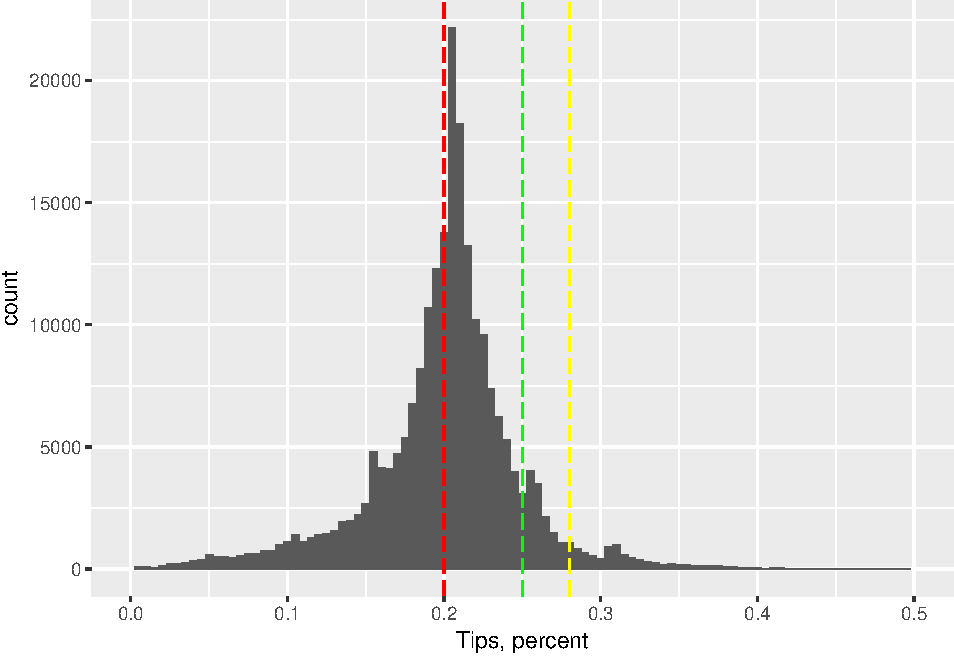
\includegraphics{thesis_files/figure-latex/tip-region-1.pdf} Figure
\ref{fig:tip-region} is a histogram of mean tip percents for all known
pick-up and drop-off zone pairs.

\subsection{Pick-up Zone Tip
Information}\label{pick-up-zone-tip-information}

Taxi drivers are required to be indifferent to where passengers are
going. Therefore, it makes sense to investigate the average amount of
tips paid for each pick-up zone. What are the taxi pick-up zones that
have the highest tip percents?

We first calculate the average percent tip paid for each pick-up zone.
\begin{table}

\caption{\label{tab:unnamed-chunk-28}Ten taxi pick-up zones with the highest average tip without any threshold in Janaury, 2017}
\centering
\begin{tabular}[t]{rrrrrrrll}
\toprule
year & month & PULocationID & avg\_tip & num\_trips & avg\_dis & avg\_duration & Borough & Zone\\
\midrule
2017 & 1 & 176 & 0.58 & 1 & 4.32 & 17.55 & Staten Island & Oakwood\\
2017 & 1 & 30 & 0.46 & 2 & 33.70 & 136.47 & Queens & Broad Channel\\
2017 & 1 & 122 & 0.45 & 1 & 1.26 & 25.00 & Queens & Hollis\\
2017 & 1 & 86 & 0.41 & 2 & 0.28 & 1.75 & Queens & Far Rockaway\\
2017 & 1 & 15 & 0.37 & 7 & 6.57 & 14.45 & Queens & Bay Terrace/Fort Totten\\
\addlinespace
2017 & 1 & 182 & 0.36 & 7 & 5.79 & 13.76 & Bronx & Parkchester\\
2017 & 1 & 23 & 0.34 & 2 & 5.50 & 15.33 & Staten Island & Bloomfield/Emerson Hill\\
2017 & 1 & 139 & 0.33 & 5 & 25.28 & 34.98 & Queens & Laurelton\\
2017 & 1 & 117 & 0.31 & 6 & 13.42 & 82.98 & Queens & Hammels/Arverne\\
2017 & 1 & 118 & 0.30 & 1 & 0.10 & 0.70 & Staten Island & Heartland Village/Todt Hill\\
\bottomrule
\end{tabular}
\end{table}
Table @ref(tab:tip\_pickup) is a list of pick-up zones with their
average percent tip.

Below is a histogram of average percent tips paid for all pick-up zones.
\begin{verbatim}
Warning: Removed 3 rows containing non-finite values (stat_bin).
\end{verbatim}
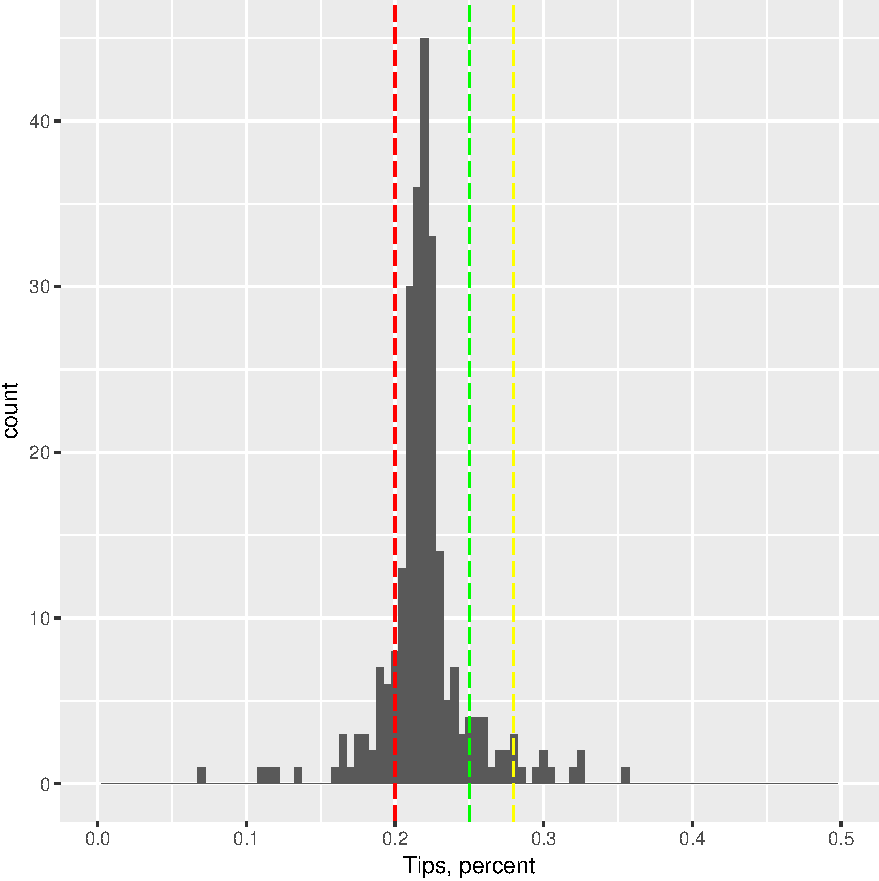
\includegraphics{thesis_files/figure-latex/pickup-vis-1.pdf} As show in
Figure \ref{fig:pickup-vis}, the first peak is around 20\%, which is the
cheapest default option on the touch panel for passengers to chose.

\textbf{Does trip distance increase the percent tips paid?} One of the
questions that I always wonder is whether longer trips result in higher
tip percent. It takes taxi drivers more time to complete longer trips,
so passengers might want to compensate taxi drivers more. I personally
pay higher percent of tips for longer rides, so I believe trip distance
has an impact on percentage of tips paid.
\begin{verbatim}
                Estimate   Std. Error   t value Pr(>|t|)
(Intercept)  0.211325482 3.733048e-04 566.09360        0
avg_dis     -0.001052903 2.105014e-05 -50.01881        0
\end{verbatim}
Acoording to the simple linear regression result, trip distance does
have a negative significant impact on the percent of tips paid,
controlling for both pick-up and drop-off locations. This could be
caused by a psycological reason. Long trips cost more than short trips.
For a constant tip percent, the absolute value of tip amount cost more
for longer trips. For example, for a \$100 trip, 20\% tip costs \$20;
for a \$50 trip, 20\% tip costs \$10. Even though consumers are paying
the same percent amount of tips, \$20 is more expensive than \$10.
Therefore, consumers might decide to pay less percent tip for longer
trips.

\subsection{Which taxi zones have the highest number of
pick-ups?}\label{which-taxi-zones-have-the-highest-number-of-pick-ups}

Let's fist take a look at which pick-up zones have the highest number of
pick-ups.

We can create a heat map to visulizae the number of trip for each
pick-up zones on a map of New York City Taxi Zones.
\begin{figure}

{\centering 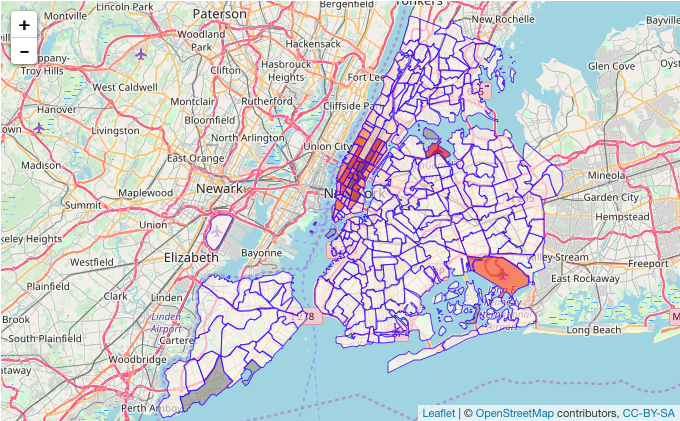
\includegraphics[width=4.96in]{figure/num_trip} 

}

\caption{Number of Pick-ups in Each Taxi Zone}\label{fig:num-trip}
\end{figure}
According to Figure \ref{fig:num-trip}, It's obivous that Upper East
Side Manhattan, Midtown Manhattan, and La Guardia Airport are the most
popular location for pick-ups.
\begin{table}

\caption{\label{tab:unnamed-chunk-32}Ten taxi zones with the highest number of pick-ups}
\centering
\begin{tabular}[t]{r|r|r|r|r|l|l}
\hline
PULocationID & avg\_tip & num\_trips & avg\_dis & avg\_duration & Borough & Zone\\
\hline
237 & 0.20 & 2519900 & 9.21 & 33.32 & Manhattan & Upper East Side South\\
\hline
161 & 0.21 & 2461602 & 10.04 & 34.48 & Manhattan & Midtown Center\\
\hline
234 & 0.20 & 2382970 & 9.63 & 33.22 & Manhattan & Union Sq\\
\hline
236 & 0.20 & 2372509 & 9.21 & 31.94 & Manhattan & Upper East Side North\\
\hline
162 & 0.21 & 2349386 & 9.70 & 32.83 & Manhattan & Midtown East\\
\hline
170 & 0.21 & 2231723 & 9.66 & 31.90 & Manhattan & Murray Hill\\
\hline
186 & 0.21 & 2193036 & 9.99 & 36.77 & Manhattan & Penn Station/Madison Sq West\\
\hline
79 & 0.20 & 2097416 & 9.48 & 30.39 & Manhattan & East Village\\
\hline
138 & 0.21 & 2059444 & 11.90 & 36.10 & Queens & LaGuardia Airport\\
\hline
230 & 0.20 & 1972303 & 10.32 & 35.97 & Manhattan & Times Sq/Theatre District\\
\hline
\end{tabular}
\end{table}
Table @ref(tab:tip\_pickup\_zone) gives you a better idea of which taxi
zones have the highest number of pick-ups.

\subsection{Which taxi zones have the highest percent
tips?}\label{which-taxi-zones-have-the-highest-percent-tips}

Most yellow cab pick-ups occur in Manhattan. If we focus on the pick-up
zones that have at least 30 trips per day or 10950 per year, we will
observe that many taxi pick-up zones with highest percent tips are not
necessarily the ones with the highest number of pick-ups.
\begin{Shaded}
\begin{Highlighting}[]
\CommentTok{# pick a threshold for the cutoff number of trips}
\NormalTok{pickup_zone_}\DecValTok{30}\NormalTok{ <-}\StringTok{ }\NormalTok{tip_pickup_zone }\OperatorTok\StringTok{ }\KeywordTok{filter}\NormalTok{(num_trips }\OperatorTok{>=}\StringTok{ }\NormalTok{(}\DecValTok{30} \OperatorTok{*}\StringTok{ }
\StringTok{    }\DecValTok{365}\NormalTok{)) }\OperatorTok\StringTok{ }\KeywordTok{arrange}\NormalTok{(}\KeywordTok{desc}\NormalTok{(avg_tip))}
\end{Highlighting}
\end{Shaded}
\begin{table}

\caption{\label{tab:unnamed-chunk-34}Ten taxi pick-up zones with the highest percent tip (taxi zones has at least 30 pick-up per day)}
\centering
\begin{tabular}[t]{r|r|r|r|r|l|l}
\hline
PULocationID & avg\_tip & num\_trips & avg\_dis & avg\_duration & Borough & Zone\\
\hline
10 & 0.22 & 13329 & 14.27 & 42.94 & Queens & Baisley Park\\
\hline
161 & 0.21 & 2461602 & 10.04 & 34.48 & Manhattan & Midtown Center\\
\hline
162 & 0.21 & 2349386 & 9.70 & 32.83 & Manhattan & Midtown East\\
\hline
170 & 0.21 & 2231723 & 9.66 & 31.90 & Manhattan & Murray Hill\\
\hline
186 & 0.21 & 2193036 & 9.99 & 36.77 & Manhattan & Penn Station/Madison Sq West\\
\hline
138 & 0.21 & 2059444 & 11.90 & 36.10 & Queens & LaGuardia Airport\\
\hline
13 & 0.21 & 704925 & 10.22 & 32.82 & Manhattan & Battery Park City\\
\hline
261 & 0.21 & 363915 & 10.02 & 33.07 & Manhattan & World Trade Center\\
\hline
88 & 0.21 & 268535 & 10.26 & 33.44 & Manhattan & Financial District South\\
\hline
33 & 0.21 & 72911 & 7.33 & 26.85 & Brooklyn & Brooklyn Heights\\
\hline
\end{tabular}
\end{table}
People might think it is more reasonable to ses a list that is populated
with Zones in Manhattan, since that's where all the wealthy people live.
However, Table @ref(tab:pickup\_zone\_30) shows that passengers who get
on taxis from certain zones in Brooklyn and Queens also pay a lot of
tips. Taxi drivers who would love to get more tips compensation can
drive to the zones listed above to pick-up passengers.

If we focus on the pick-up zones that have more than 3000 trips per day,
then we observe that all pick-up zones that have the highest percent
tips are in Manhattan besides La Guardia Airport.
\begin{Shaded}
\begin{Highlighting}[]
\NormalTok{pickup_zone_}\DecValTok{3000}\NormalTok{ <-}\StringTok{ }\NormalTok{tip_pickup_zone }\OperatorTok\StringTok{ }\KeywordTok{filter}\NormalTok{(num_trips }\OperatorTok{>=}\StringTok{ }\NormalTok{(}\DecValTok{365} \OperatorTok{*}\StringTok{ }
\StringTok{    }\DecValTok{3000}\NormalTok{)) }\OperatorTok\StringTok{ }\KeywordTok{arrange}\NormalTok{(}\KeywordTok{desc}\NormalTok{(avg_tip))}
\end{Highlighting}
\end{Shaded}
\begin{table}

\caption{\label{tab:unnamed-chunk-36}Ten taxi pick-up zones with the highest percent tip  (taxi zones has at least 3000 pick-up per day)}
\centering
\begin{tabular}[t]{r|r|r|r|r|l|l}
\hline
PULocationID & avg\_tip & num\_trips & avg\_dis & avg\_duration & Borough & Zone\\
\hline
161 & 0.21 & 2461602 & 10.04 & 34.48 & Manhattan & Midtown Center\\
\hline
162 & 0.21 & 2349386 & 9.70 & 32.83 & Manhattan & Midtown East\\
\hline
170 & 0.21 & 2231723 & 9.66 & 31.90 & Manhattan & Murray Hill\\
\hline
186 & 0.21 & 2193036 & 9.99 & 36.77 & Manhattan & Penn Station/Madison Sq West\\
\hline
138 & 0.21 & 2059444 & 11.90 & 36.10 & Queens & LaGuardia Airport\\
\hline
237 & 0.20 & 2519900 & 9.21 & 33.32 & Manhattan & Upper East Side South\\
\hline
234 & 0.20 & 2382970 & 9.63 & 33.22 & Manhattan & Union Sq\\
\hline
236 & 0.20 & 2372509 & 9.21 & 31.94 & Manhattan & Upper East Side North\\
\hline
79 & 0.20 & 2097416 & 9.48 & 30.39 & Manhattan & East Village\\
\hline
230 & 0.20 & 1972303 & 10.32 & 35.97 & Manhattan & Times Sq/Theatre District\\
\hline
\end{tabular}
\end{table}
There are more than 100 times more yellow cab pick-ups that happen in
Manhattan everyday than in Brooklyn. By comparing the average tip
percent in Table @ref(tab:pickup\_zone\_30) and Table
@ref(tab:pickup\_zone\_3000), we can observe that percent tips paid in
taxi zones with low pick-up numbers seem to be higher than percent tips
paid in taxi zones with high pick-up numbers.

\section{What features of taxi trips are attractive to taxi
drivers?}\label{what-features-of-taxi-trips-are-attractive-to-taxi-drivers}

So far, we have learned what pick-up zones offer the highest percent
tip. Now, we want to dig into the relationships between percent tip and
taxi-zone-specific variables.

\subsection{Do taxi drivers tend to go to zones that offer high
tips?}\label{do-taxi-drivers-tend-to-go-to-zones-that-offer-high-tips}

It is not easy to find an available taxi on the street on New York City,
because the demand for taxi trips is much higher than the supply. Does
paying high percent tips help customers to attract more taxis? If
customers from certain regions keep paying higher tips, taxi drivers
might be able to learn from their experiences in those regions, and be
willing to wonder around those regions more often and pick up
passengers. Pick-up zones with higher tips should attract more taxi
drivers with the control of taxi zones. However, conflivting to what I
assumed, Table @ref(tab:pickup\_zone\_30) and Table
@ref(tab:pickup\_zone\_3000) show that percent tips seem to have a
inverse relationship with number of pick-ups.

Let's test the relationship between number of trips and average percent
tips in each pick-up zone:
\begin{verbatim}
             Estimate Std. Error   t value     Pr(>|t|)
(Intercept)   61203.5   6818.591  8.975975 5.106658e-19
avg_tip     -166807.7  27124.605 -6.149682 8.900927e-10
\end{verbatim}
Each one percent increase in average tips in pick-up zones is associated
with a significant decline in the number of trips per month. Therefore,
increase in average percent tips in pick-up zones does not make pick-up
zones more attractive. Taxi drivers are not attracted to taxi zones with
high percent tips. This is why we observe high percent tips in Baisley
Park, Queens in Table @ref(tab:pickup\_zone\_30).

\subsection{Do passengers pay more tips during rush
hours?}\label{do-passengers-pay-more-tips-during-rush-hours}

New York City Taxi Fare \& Limousine Commission has information on how
New York City taxi fare amount is calculated on their
\href{http://www.nyc.gov/html/tlc/html/passenger/taxicab_rate.shtml}{official
website}.

\textbf{Metered Fare Information} \textbf{Onscreen rate is `Rate \#01 --
Standard City Rate.'} \emph{The initial charge is \$2.50. }Plus 50 cents
per 1/5 mile or 50 cents per 60 seconds in slow traffic or when the
vehicle is stopped. \emph{In moving traffic on Manhattan streets, the
meter should ``click'' approximately every four downtown blocks, or one
block going cross-town (East-West). }There is a 50-cent MTA State
Surcharge for all trips that end in New York City or Nassau, Suffolk,
Westchester, Rockland, Dutchess, Orange or Putnam Counties. \emph{There
is a 30-cent Improvement Surcharge. }There is a daily 50-cent surcharge
from 8pm to 6am. \emph{There is a \$1 surcharge from 4pm to 8pm on
weekdays, excluding holidays. }Passengers must pay all bridge and tunnel
tolls. \emph{Your receipt will show your total fare including tolls.
Please take your receipt. }The driver is not required to accept bills
over \$20. \emph{Please tip your driver for safety and good service.
}There are no charges for extra passengers or bags.

In taxi fare calculation, the only unknown variable is slow-trafice
time, and all other variables were collected by the meters installed on
each medallion taxi for each trip. It is reasonable to assume that for
trips with the same pick-up and drop-off locations, the longer the total
slow traffic time is, the longer the trip would take. Taxi drivers are
compensated for both the normal-speed trip distance and the time spent
in slow-traffice. According to the fare calculation algorithm, in moving
traffic on Manhattan streets, the meter should ``click'' approximately
every four downtown blocks, or one block going cross-town (East-West);
in slow traffic, the meter should ``click'' every 60 seconds. Therefore,
slow traffic increase the minute per mile ratio.

New York City has the worst traffic jam, and it has overtaken Miami to
be voted the U.S. city with the angriest and most aggressive drivers in
2009, according to a survey on road rage released on Tuesday. Bad
traffic also cause slow-traffic, and taxi drivers tend to suck in
traffic during rush hours.(Reaney, 2009) Does minute per mile ratio have
an impact on the percent tip that passengers pay? Do passengers
compensate taxi drivers more during rush hours? Are passengers
sympathetic to taxi drivers for the time they spend in slow traffic?
\begin{verbatim}
                Estimate   Std. Error   t value Pr(>|t|)
(Intercept)  0.193453599 1.870711e-04 1034.1180        0
min_per_mile 0.002841351 3.134322e-05   90.6528        0
\end{verbatim}
As shown in the regression result, fare per minute ratio has a
significant positive impact on percent tip. \texttt{min\_per\_mile}
ratio does have an positive impact on percent tips. Since trips with
slow traffice can be depicted by high minute per mile ratio, passengers
do pay more tips during rush hours.

\chapter{New York City Taxi Passengers}\label{chapter4}

\section{How long does it take to get to JFK, La Guardia, and Newark
Airports? When is the best time to
depart?}\label{how-long-does-it-take-to-get-to-jfk-la-guardia-and-newark-airports-when-is-the-best-time-to-depart}

We want to calculate the average number of minutes it takes to go to all
three airport from a specific taxi zone at every hour. First, we want to
focus on trips going to any of the three airports, JFK, LaGuardia, or
Newark Airport. We need to load trip records with destination as one of
the three airports from the MySQL connection we built.
\begin{Shaded}
\begin{Highlighting}[]
\NormalTok{to_jfk_trip <-}\StringTok{ }\NormalTok{taxi }\OperatorTok\StringTok{ }\KeywordTok{tbl}\NormalTok{(}\StringTok{"yellow"}\NormalTok{) }\OperatorTok\StringTok{ }\KeywordTok{filter}\NormalTok{(DOLocationID }\OperatorTok{==}\StringTok{ }
\StringTok{    }\DecValTok{132}\NormalTok{) }\OperatorTok\StringTok{ }\KeywordTok{collect}\NormalTok{(}\DataTypeTok{n =} \OtherTok{Inf}\NormalTok{)}

\NormalTok{to_lg_trip <-}\StringTok{ }\NormalTok{taxi }\OperatorTok\StringTok{ }\KeywordTok{tbl}\NormalTok{(}\StringTok{"yellow"}\NormalTok{) }\OperatorTok\StringTok{ }\KeywordTok{filter}\NormalTok{(DOLocationID }\OperatorTok{==}\StringTok{ }
\StringTok{    }\DecValTok{138}\NormalTok{) }\OperatorTok\StringTok{ }\KeywordTok{collect}\NormalTok{(}\DataTypeTok{n =} \OtherTok{Inf}\NormalTok{)}

\NormalTok{to_newark_trip <-}\StringTok{ }\NormalTok{taxi }\OperatorTok\StringTok{ }\KeywordTok{tbl}\NormalTok{(}\StringTok{"yellow"}\NormalTok{) }\OperatorTok\StringTok{ }\KeywordTok{filter}\NormalTok{(DOLocationID }\OperatorTok{==}\StringTok{ }
\StringTok{    }\DecValTok{1}\NormalTok{) }\OperatorTok\StringTok{ }\KeywordTok{collect}\NormalTok{(}\DataTypeTok{n =} \OtherTok{Inf}\NormalTok{)}
\end{Highlighting}
\end{Shaded}
Now we want to calculate the average amount of time it take from each
zone to one of the three airports during each hour.

So far, we have created three tables summarsing the average number of
minutes it takes to go to all three airports for every hour from
different taxi zones.

It would be easier if we combine all three tables and put information
related to trip duration to all three airports in the same table.
\begin{table}

\caption{\label{tab:unnamed-chunk-46}Average number of minutes it takes from Alphabet City, Manhattan to JFK Airport during different hours}
\centering
\begin{tabular}[t]{l|r|r|r|l}
\hline
  & PULocationID & hour & avg\_min & airport\\
\hline
10 & 4 & 0 & 45.37000 & JFK\\
\hline
11 & 4 & 1 & 36.77500 & JFK\\
\hline
12 & 4 & 2 & 28.66000 & JFK\\
\hline
13 & 4 & 3 & 27.83350 & JFK\\
\hline
14 & 4 & 4 & 27.19490 & JFK\\
\hline
15 & 4 & 5 & 28.68889 & JFK\\
\hline
16 & 4 & 6 & 34.25271 & JFK\\
\hline
17 & 4 & 7 & 38.13817 & JFK\\
\hline
18 & 4 & 8 & 41.59687 & JFK\\
\hline
19 & 4 & 9 & 35.39226 & JFK\\
\hline
20 & 4 & 10 & 36.22867 & JFK\\
\hline
\end{tabular}
\end{table}
Table @ref(tab:three\_air) displays the average number of minutes it
takes from Alphabet City, Manhattan to JFK Airport during different
hours.

\subsection{Case Study: From Alphabet City, Manhattan to all three
airport}\label{case-study-from-alphabet-city-manhattan-to-all-three-airport}

Alphabet City, Manhattan has pick-up zone ID number 4. Let's take a look
at how much time is needed to travel to all three airports from taxi
zone No.4.
\begin{Shaded}
\begin{Highlighting}[]
\NormalTok{alphabet <-}\StringTok{ }\NormalTok{three_air }\OperatorTok\StringTok{ }\KeywordTok{filter}\NormalTok{(PULocationID }\OperatorTok{==}\StringTok{ }\DecValTok{4}\NormalTok{)}
\end{Highlighting}
\end{Shaded}
\begin{figure}
\centering
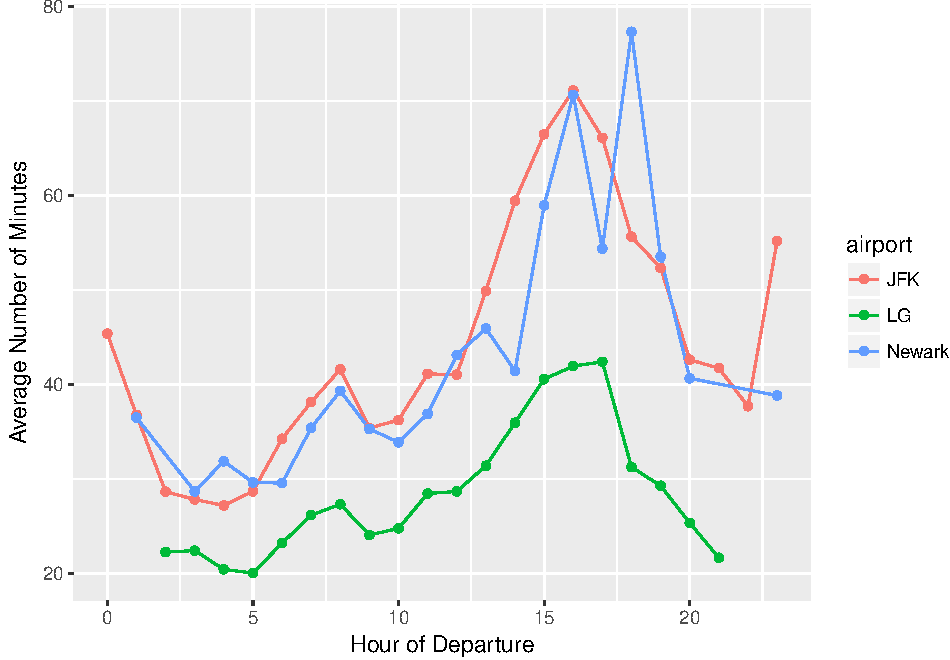
\includegraphics{thesis_files/figure-latex/airport-vis-1.pdf}
\caption{\label{fig:airport-vis}Average number of minutes it takes from
Alphabet City, Manhattan to all three airports during different hours}
\end{figure}
According to the red line Figure \ref{fig:airport-vis}, it takes the
least time, less than 30 minutes, to travel from Alphabet City,
Manhattan to JFK Airport around 4 AM in the morning, and it takes the
most time, about 70 minutes, around 4 PM in the afternoon.

According to the green line, it takes the least time, about 20 minutes,
to travel to JFK Airport around 5 AM in the morning, and it takes the
most time, more than 40 minutes, around 5 PM in the afternoon.

As shown by the blue line, it takes the least time, a little less than
30 minutes, to travel to Newark Airport at 2 AM at midnight, and it
takes the most time, a little less than 80 minutes, around 6 PM in the
evening.

\subsection{A Shiny App: allowing users to choose a pick up zone of
their interest, and output the best time to travel from that zone to all
three airports in New
York}\label{a-shiny-app-allowing-users-to-choose-a-pick-up-zone-of-their-interest-and-output-the-best-time-to-travel-from-that-zone-to-all-three-airports-in-new-york}
\begin{center}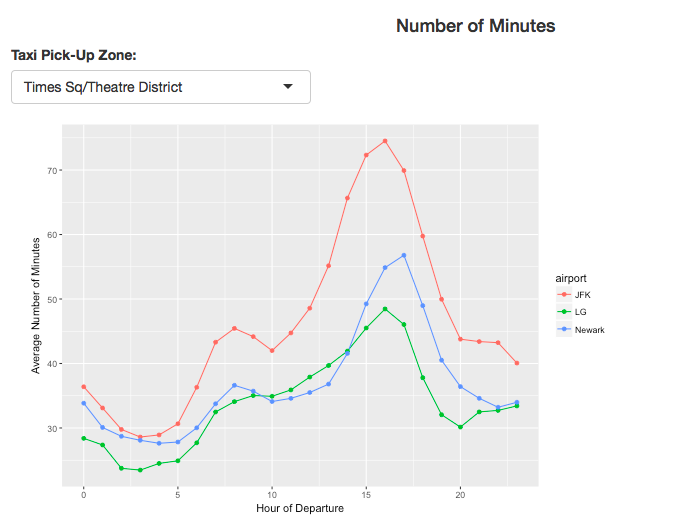
\includegraphics[width=3.37in]{figure/shinyapp} \end{center}

This Shiny App helps passengers to estimate the amount of time that is
needed for them to travel to any one of the these three airports from
any New York City taxi zones.

\section{How does weather affect the number of taxi and Lyft
trips?}\label{how-does-weather-affect-the-number-of-taxi-and-lyft-trips}

On a snowy or rainy day, it is hard for passengers to find a yellow cab
on the street. Taxi drivers get paid at the same rate no matter how bad
the weather gets, so they tend to stay at home instead of going out to
work when the weather is bad. Uber drivers, however, get paid more on a
snowy or rainy day, since Uber uses a pricing model that takes the
number of Uber vehicles available on the street into account. When
weather is bad, less Uber vehicles are available on the street, so Uber
fare rate increases. Uber's pricing model gives Uber drivers an
incentive to keep working on ugly days. Lyft has a similar pricing model
to the one that Uber uses.

In this section, we want to study the number of pickups of yellow cab,
Uber, and Lyft. We compare number of pick-ups in each taxi zone in the
weeks of bad weather with previous weeks' total number of pick-ups to
see whether Uber drivers have an incentive to drive around the city more
when weather gets bad.

\textbf{Uber Weekly Data}
\begin{table}

\caption{\label{tab:unnamed-chunk-51}Uber 2017 Weekly Total Dispatched Trips}
\centering
\begin{tabular}[t]{l|l|r}
\hline
Pickup Start Date & Pickup End Date & Total Dispatched Trips\\
\hline
01/01/2017 & 01/07/2017 & 2866569\\
\hline
01/08/2017 & 01/14/2017 & 3114792\\
\hline
01/15/2017 & 01/21/2017 & 3089595\\
\hline
01/22/2017 & 01/28/2017 & 3299763\\
\hline
01/29/2017 & 02/04/2017 & 3224451\\
\hline
02/05/2017 & 02/11/2017 & 3310481\\
\hline
02/12/2017 & 02/18/2017 & 3456042\\
\hline
02/19/2017 & 02/25/2017 & 3194805\\
\hline
02/26/2017 & 03/04/2017 & 3533347\\
\hline
03/05/2017 & 03/11/2017 & 3614559\\
\hline
\end{tabular}
\end{table}
\textbf{Yellow Cab Weekly Data}
\begin{table}

\caption{\label{tab:unnamed-chunk-54}Yellow Taxi 2017 Weekly Total Dispatched Trips}
\centering
\begin{tabular}[t]{l|r}
\hline
Pickup Start Date & Total Dispatched Trips\\
\hline
2017-01-01 & 2044643\\
\hline
2017-01-08 & 2230950\\
\hline
2017-01-15 & 2219214\\
\hline
2017-01-22 & 2307122\\
\hline
2017-01-29 & 2331749\\
\hline
2017-02-05 & 2181622\\
\hline
2017-02-12 & 2387399\\
\hline
2017-02-19 & 2225850\\
\hline
2017-02-26 & 2464800\\
\hline
2017-03-05 & 2456285\\
\hline
\end{tabular}
\end{table}
In this section, we use New York City Yellow Taxi and Uber data to
calculate the number of trips occurred in each week.

\subsection{Case Study: March 14th, 2017 Snow
Storm}\label{case-study-march-14th-2017-snow-storm}

There are two commonly known bad weather consitions, rainy and snowy
day. Let's first focus on snowstorm. I downloaded daily Central Park
weather data from the National Climatic Data Center, and joined it to
the taxi data to see if we could learn anything else about the
relationship between weather and taxi rides.

On March 14th, 2017, a snow storm brought seven inches of snow to New
York City. \textbf{Yellow Taxi}
\begin{verbatim}
  Pickup Start Date Total Dispatched Trips
1        2017-03-05                2456285
2        2017-03-12                2066285
\end{verbatim}
\begin{Shaded}
\begin{Highlighting}[]
\NormalTok{(}\DecValTok{2066285} \OperatorTok{-}\StringTok{ }\DecValTok{2456285}\NormalTok{)}\OperatorTok{/}\DecValTok{2456285}
\end{Highlighting}
\end{Shaded}
\begin{verbatim}
[1] -0.1587764
\end{verbatim}
\textbf{Uber}
\begin{verbatim}
# A tibble: 2 x 3
# Groups:   Pickup Start Date [2]
  `Pickup Start Date` `Pickup End Date` `Total Dispatched Trips`
                <chr>             <chr>                    <int>
1          03/05/2017        03/11/2017                  3614559
2          03/12/2017        03/18/2017                  3430189
\end{verbatim}
\begin{Shaded}
\begin{Highlighting}[]
\NormalTok{(}\DecValTok{3430189} \OperatorTok{-}\StringTok{ }\DecValTok{3614559}\NormalTok{)}\OperatorTok{/}\DecValTok{3614559}
\end{Highlighting}
\end{Shaded}
\begin{verbatim}
[1] -0.05100761
\end{verbatim}
In this case, we observe that the percent decline in Uber's total number
of pick-ups is 10\% less than the percent decline in Yellow Taxi's total
number of dropp-off. Even though the total number of Uber pick-ups did
not increase, Uber's pricing model definitely was able to keep more
drivers in the market on a snowy day.

\textbf{More analysis is needed here}

\chapter{New York City Taxi Fare \& Limousine
Commission}\label{chapter5}

\section{Should there be a flat rate between Manhattan and John F.
Kennedy International
Airport?}\label{should-there-be-a-flat-rate-between-manhattan-and-john-f.-kennedy-international-airport}

Why is there a flat rate to and from JFK airport and any location in
Manhattan? Why is the flat rate \$52? Does TLC make profit from the \$52
flat rate? Does \$52 reduce the cogestion on the road to JFK airport and
make taking a train a more preferable choice? The New York City taxi
trip records can reveal the answers to these questions.

Imagine it's your first time travelling to New York City, and you
decided to live in a hotel in Manhattan Since you do not know much about
the city, the \$52 flat rate is nice for you, and it incentivizes you to
take taxi to the JFK Airport. If there is no flat rate, there is
uncertainty in how much someone needs to pay to take a taxi to JFK, and
tourists might instead choose to take the train, even though taking a
train would cost them more time and inconvenience.

Additionally, people who are native to Manhattan would have paid more
than \$52 to take a taxi to go to the JFK Airport. The higher the taxi
fare is, the less the demand for taxi will be. Therefore, having a flat
rate,helps taxi drivers to get more trips from Manhattan to JFK Airport.

\subsection{People in Manhattan benefit from the \$52 flat
rate.}\label{people-in-manhattan-benefit-from-the-52-flat-rate.}

If there is no flat rate between JFK and Manhattan, how much would
passengers pay for the distance they travelled between JFK Airport AND
Manhattan? And how much more or less should they have paid comparing to
the \$52 flat rate?

In this study, we are only interested in yellow taxi trip between
Manhattan and JFK Airport.
\begin{Shaded}
\begin{Highlighting}[]
\NormalTok{jfk_trip_raw <-}\StringTok{ }\NormalTok{taxi }\OperatorTok\StringTok{ }\KeywordTok{tbl}\NormalTok{(}\StringTok{"yellow"}\NormalTok{) }\OperatorTok\StringTok{ }\KeywordTok{filter}\NormalTok{(RatecodeID }\OperatorTok{==}\StringTok{ }
\StringTok{    }\DecValTok{2}\NormalTok{) }\OperatorTok\StringTok{ }\KeywordTok{collect}\NormalTok{(}\DataTypeTok{n =} \OtherTok{Inf}\NormalTok{)}
\end{Highlighting}
\end{Shaded}
\begin{verbatim}

Read 17.1% of 1581568 rows
Read 41.1% of 1581568 rows
Read 53.1% of 1581568 rows
Read 62.6% of 1581568 rows
Read 82.8% of 1581568 rows
Read 85.4% of 1581568 rows
Read 1581568 rows and 20 (of 20) columns from 0.175 GB file in 00:00:09
\end{verbatim}
\textbf{Trips from Manhattan to JFK Airport} We first focus on all the
trips that departed in Manhattan and went to JFK Airport, and then we
calculate the estmated fare amount that the passengers should have paid
based on the distance travelled from each pick-up point to JFK Airport
based on the fare rate suggested by TLC for each pick-up zone.

Here is a map of estmated fare amount calculated by taking the average
of all estimated fare amounts from the same pick-up zone to JFK Airport
based on the fare rate suggested by TLC for each pick-up zone.
\begin{figure}

{\centering 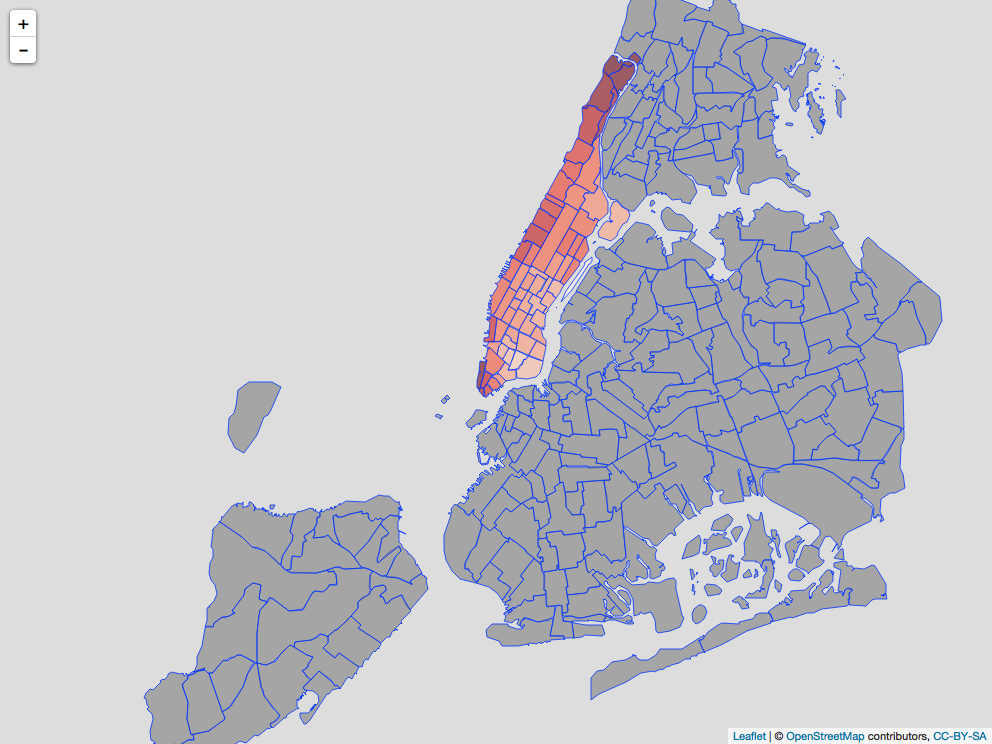
\includegraphics[width=4.96in]{figure/to_jkf_fare_vis} 

}

\caption{Estmated fare amount from the each pick-up zone to JFK Airport}\label{fig:to-jkf-fare-vis}
\end{figure}
According to the map, trips from Midtown on average cost less than trips
from other taxi zones in Manhattan.

\subsection{Taxi zones pays on average more than
\$52}\label{taxi-zones-pays-on-average-more-than-52}
\begin{table}

\caption{\label{tab:unnamed-chunk-65}Ten pick-up zones with the highest avergae fare from Manhattan to JKF Airport}
\centering
\begin{tabular}[t]{r|r|r|r|l|l}
\hline
LocationID & num\_trips & avg\_est\_fare & avg\_est\_diff & Borough & Zone\\
\hline
105 & 3 & 66.38167 & 14.381667 & Manhattan & Governor's Island/Ellis Island/Liberty Island\\
\hline
128 & 3 & 64.53667 & 12.536667 & Manhattan & Inwood Hill Park\\
\hline
153 & 1 & 64.51000 & 12.510000 & Manhattan & Marble Hill\\
\hline
127 & 35 & 64.08814 & 12.088143 & Manhattan & Inwood\\
\hline
13 & 10209 & 64.00873 & 12.009420 & Manhattan & Battery Park City\\
\hline
243 & 125 & 63.05100 & 11.051000 & Manhattan & Washington Heights North\\
\hline
12 & 272 & 62.15925 & 10.159246 & Manhattan & Battery Park\\
\hline
120 & 7 & 62.06714 & 10.067143 & Manhattan & Highbridge Park\\
\hline
244 & 535 & 60.36664 & 8.366645 & Manhattan & Washington Heights South\\
\hline
239 & 12515 & 60.17096 & 8.170965 & Manhattan & Upper West Side South\\
\hline
\end{tabular}
\end{table}
Let's visualize the taxi zones that would have costed more than the \$52
flat rate.

\textbackslash{}begin\{figure\}

\{\centering 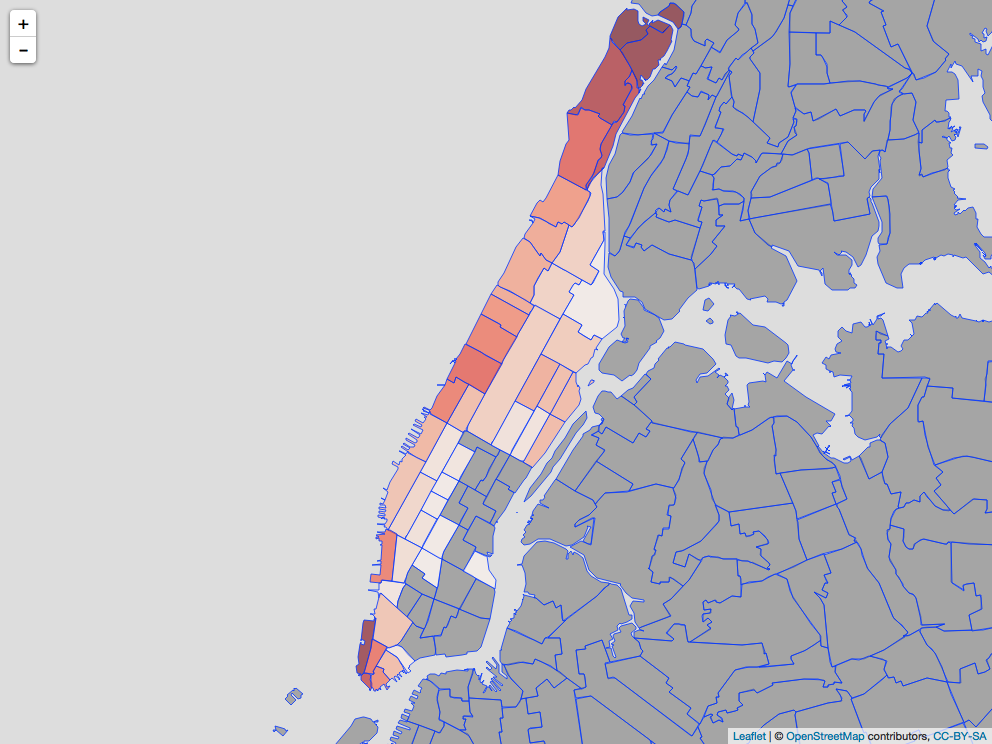
\includegraphics[width=4.96in]{figure/to_jfk_fare_above_vis}

\}

\textbackslash{}caption\{Zones that cost more than the \$52 flat
rate\}(\#fig:num-to\_jfk\_fare\_above\_vis)
\textbackslash{}end\{figure\}

Therefore, passengers from places in Manhattan besides Midtown, East
Village, and some parts of Lower Manhattan benefit from the \$52 flat
rate. However, people living in Midtown, East Village, and some parts of
Lower Manhattan might be relatively more indifferent to the price of
taxi. Instead, they probably put more emphasis on convenience and time.
\begin{Shaded}
\begin{Highlighting}[]
\KeywordTok{mean}\NormalTok{(to_jkf_zone}\OperatorTok{$}\NormalTok{avg_est_diff)}
\end{Highlighting}
\end{Shaded}
\begin{verbatim}
[1] 2.947066
\end{verbatim}
On average people travel from Manhattan pay \$2.14 less with the \$52
flat rate policy. Therefore, passengers overall benefit from the \$52
flat rate policy.

\section{However, are taxi drivers happy when their passengers are going
to JFK Airport from
Manhattan?}\label{however-are-taxi-drivers-happy-when-their-passengers-are-going-to-jfk-airport-from-manhattan}

Everytime I travel to New York City, I always take Yellow cabs to go
around the city. It seemed to me that the cab drivers were always happy
whenever they heard me telling them that I need to go to the JFK Airport
from Manhattan. Are taxi drivers happy when their passengers are going
to JFK Airport from Manhattan? How much on average would taxi driver
make on their way bavk to the city from Manhattan?
\begin{Shaded}
\begin{Highlighting}[]
\NormalTok{from_jfk <-}\StringTok{ }\NormalTok{jfk_trip_flat }\OperatorTok\StringTok{ }\KeywordTok{filter}\NormalTok{(PULocationID }\OperatorTok{==}\StringTok{ }\DecValTok{132}\NormalTok{) }\OperatorTok\StringTok{ }
\StringTok{    }\KeywordTok{mutate}\NormalTok{(}\DataTypeTok{est_fare =} \FloatTok{2.5} \OperatorTok{+}\StringTok{ }\FloatTok{0.5} \OperatorTok{*}\StringTok{ }\NormalTok{trip_distance }\OperatorTok{*}\StringTok{ }\DecValTok{5} \OperatorTok{+}\StringTok{ }\NormalTok{extra }\OperatorTok{+}\StringTok{ }
\StringTok{        }\NormalTok{improvement_surcharge }\OperatorTok{+}\StringTok{ }\NormalTok{mta_tax }\OperatorTok{+}\StringTok{ }\NormalTok{tolls_amount) }\OperatorTok\StringTok{ }\KeywordTok{mutate}\NormalTok{(}\DataTypeTok{est_diff =}\NormalTok{ est_fare }\OperatorTok{-}\StringTok{ }
\StringTok{    }\NormalTok{fare_amount) }\OperatorTok\StringTok{ }\KeywordTok{rename}\NormalTok{(}\DataTypeTok{LocationID =}\NormalTok{ DOLocationID) }\OperatorTok\StringTok{ }\KeywordTok{left_join}\NormalTok{(taxi_zone_lookup, }
    \DataTypeTok{by =} \StringTok{"LocationID"}\NormalTok{)}
\end{Highlighting}
\end{Shaded}
Since a taxi driver coming from Manhattan to JFK Airport could be
directed back to anywhere in the city. We can calculate the average taxi
fare amount that the taxi drivers would get paid for a random trip from
JFK Airport to any part of the city.
\begin{Shaded}
\begin{Highlighting}[]
\KeywordTok{mean}\NormalTok{(from_jfk}\OperatorTok{$}\NormalTok{est_fare)}
\end{Highlighting}
\end{Shaded}
\begin{verbatim}
[1] 55.77144
\end{verbatim}
On average, taxi drivers would get paid for \$55.77 for a trip from the
JFK Airport to any taxi zone in Manhattan. What are the most popular
drop-off zones for yellow taxis from JFK Airport?
\begin{table}

\caption{\label{tab:unnamed-chunk-71}Ten most popular destinations in Manhattan}
\centering
\begin{tabular}[t]{r|r|r|r|l|l}
\hline
LocationID & num\_trips & avg\_est\_fare & avg\_est\_diff & Borough & Zone\\
\hline
230 & 59128 & 55.67270 & 3.6727027 & Manhattan & Times Sq/Theatre District\\
\hline
162 & 40337 & 53.53283 & 1.5328320 & Manhattan & Midtown East\\
\hline
170 & 39846 & 52.63733 & 0.6373336 & Manhattan & Murray Hill\\
\hline
164 & 38704 & 53.81057 & 1.8105702 & Manhattan & Midtown South\\
\hline
161 & 36229 & 54.60352 & 2.6035182 & Manhattan & Midtown Center\\
\hline
48 & 35104 & 55.98070 & 3.9806952 & Manhattan & Clinton East\\
\hline
163 & 34380 & 54.84415 & 2.8441508 & Manhattan & Midtown North\\
\hline
79 & 26399 & 53.23628 & 1.2362819 & Manhattan & East Village\\
\hline
239 & 24609 & 61.19056 & 9.1905555 & Manhattan & Upper West Side South\\
\hline
107 & 22929 & 54.15960 & 2.1595981 & Manhattan & Gramercy\\
\hline
\end{tabular}
\end{table}
Table @ref(tab:from\_jkf\_zone) shows that Times Square is the most
popular destination for passengers coming from the JFK Airport in 2017!

\textbf{What's the average fare to each dropp-off zone from JFK Airport?
}

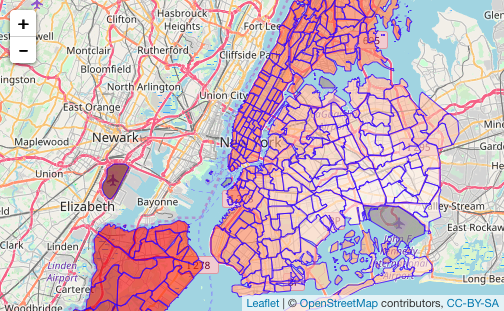
\includegraphics{figure/from_jkf_fare.png} As we expected, the red
shades are smoothly distributed, since taxi zones that are futher away
should cost more to get there.

\textbf{What's the most popular dropp-off locations for passengers from
JFK Airport? }

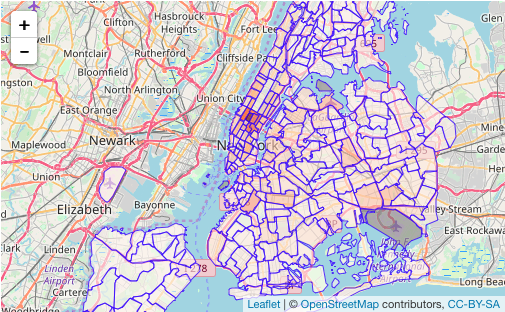
\includegraphics{figure/from_jkf_num.png} According to the map above,
Manhattan is still the most popular destination for passengers depart
from the JFK Airport.
\begin{verbatim}
# A tibble: 2 x 2
  Manhattan all_trips
      <dbl>     <int>
1         0      3691
2         1    964292
\end{verbatim}
\begin{Shaded}
\begin{Highlighting}[]
\DecValTok{964292}\OperatorTok{/}\NormalTok{(}\DecValTok{3691} \OperatorTok{+}\StringTok{ }\DecValTok{964292}\NormalTok{)}
\end{Highlighting}
\end{Shaded}
\begin{verbatim}
[1] 0.9961869
\end{verbatim}
According to the summary, the total amount of trips from JFK Airport to
Manhattan is about 99.6\% of the total number of trips travelling from
JFK Airport to all other Borough. Therefore, it is very likely for taxi
drivers to get passengers who want to go to Manhattan with a flat rate
of \$52. In this case, a round trip to and from JFK Airport is worthy.
Therefore, taxi drivers should be pretty happy when their passengers are
going to JFK Airport from Manhattan.

\chapter{Conclusion}\label{chapter5}

\section{Future Research}\label{future-research}

For future study, I would love to investigate the sharp decline in the
consumption of NYC yellow cab after e-hail services were introduced into
the NYC ride-hail market. I also want to study what the impact of
introducing new GPS and entertainment system is on the number of rides.
The global product and marketing at Verifone, Jason Gross, said that,
``I like to say that we provide what Uber says it provides.'' With the
raised expectation among rides caused by Uber and Lyft, yellow taxi
industry need to respond quickly. How does the market react to the newly
installed entertainment system? Has the market share of yellow cab
rebounded since 2016? By looking into the patterns in market shares, it
might be possible for me to predict the future market share distribution
and find out what features of ride-hail transportation are the ones that
affect market share distribution the most.

\appendix

\chapter{The First Appendix}\label{the-first-appendix}

This first appendix includes all of the R chunks of code that were
hidden throughout the document (using the \texttt{include\ =\ FALSE}
chunk tag) to help with readibility and/or setup.

\textbf{In the main Rmd file}
\begin{Shaded}
\begin{Highlighting}[]
\CommentTok{# This chunk ensures that the thesisdown package is installed}
\CommentTok{# and loaded. This thesisdown package includes the template}
\CommentTok{# files for the thesis.}
\ControlFlowTok{if}\NormalTok{ (}\OperatorTok{!}\KeywordTok{require}\NormalTok{(devtools)) }\KeywordTok{install.packages}\NormalTok{(}\StringTok{"devtools"}\NormalTok{, }\DataTypeTok{repos =} \StringTok{"http://cran.rstudio.com"}\NormalTok{)}
\ControlFlowTok{if}\NormalTok{ (}\OperatorTok{!}\KeywordTok{require}\NormalTok{(thesisdown)) devtools}\OperatorTok{::}\KeywordTok{install_github}\NormalTok{(}\StringTok{"ismayc/thesisdown"}\NormalTok{)}
\KeywordTok{library}\NormalTok{(thesisdown)}
\end{Highlighting}
\end{Shaded}
\textbf{In Chapter \ref{ref-labels}:}

\backmatter

\chapter*{References}\label{references}
\addcontentsline{toc}{chapter}{References}

\markboth{References}{References}

\noindent

\setlength{\parindent}{-0.20in} \setlength{\leftskip}{0.20in}
\setlength{\parskip}{8pt}

\hypertarget{refs}{}
\hypertarget{ref-pkgetl}{}
Baumer, B. S. (2017). A grammar for reproducible and painless
extract-transform-load operations on medium data. \emph{arXiv},
\emph{8}(23), 1--24. Retrieved from
\url{https://arxiv.org/abs/1708.07073}

\hypertarget{ref-baumer2014}{}
Baumer, B., Cetinkaya-Rundel, M., Bray, A., Loi, L., \& Horton, N. J.
(2014). R markdown: Integrating a reproducible analysis tool into
introductory statistics. \emph{arXiv Preprint arXiv:1402.1894}.

\hypertarget{ref-pkgnyctaxi}{}
Baumer, B., Li, W. P., \& Le, T. (2017). \emph{Nyctaxi: Accessing new
york city taxi data}. Retrieved from
\url{http://github.com/beanumber/nyctaxi}

\hypertarget{ref-furfaro2016}{}
Danielle Furfaro, S. C., \& Fears, D. (2016, December). NYC is already
tired of christmas and donald trump. New York Post. Retrieved from
\url{https://nypost.com/2016/12/01/nyc-is-already-tired-of-christmas-and-donald-trump/}

\hypertarget{ref-wikipedia}{}
Extract, transform, load. (2018, March). \emph{Wikipedia}. Wikimedia
Foundation. Retrieved from
\url{https://en.wikipedia.org/wiki/Extract,_transform,_load}

\hypertarget{ref-guerrini2015}{}
Guerrini, F. (2015, April). Which Is Cheaper To Use In NYC: Uber Or A
Taxi? Big Data Will Solve The Dilemma. Forbes Tech. Retrieved from
\url{https://www.forbes.com/sites/federicoguerrini/2015/04/09/living-in-new-york-this-app-will-tell-you-which-is-cheaper-uber-or-a-taxi/2/\#26bc29904023}

\hypertarget{ref-hu2017}{}
Hu, W. (2017, January). Yellow Cab, Long a Fixture of City Life, Is for
Many a Thing of the Past. The New York Times. Retrieved from
\url{https://www.nytimes.com/2017/01/15/nyregion/yellow-cab-long-a-fixture-of-city-life-is-for-many-a-thing-of-the-past.html?hp\&action=click\&pgtype=Homepage\&clickSource=story-heading\&module=second-column-region\&region=top-news\&WT.nav=top-news\&_r=0}

\hypertarget{ref-datalyft}{}
LYFT Data. (2015). NYC OpenData. Retrieved from
\url{https://data.cityofnewyork.us/Transportation/LYFT-Data/juxc-sutg/data}

\hypertarget{ref-appone}{}
OpenStreetCab. (2015). University of Cambridge UK Computer Laboratory,
University of Namur Belgium, Complexity; Networks group. Retrieved from
\url{https://www.openstreetcab.com}

\hypertarget{ref-reaney2009}{}
Reaney, P. (2009, June). New York Drivers Named Most Aggressive, Angry
in u.S. Reuters. Retrieved from
\url{https://www.reuters.com/article/us-driving-roadrage-life/new-york-drivers-named-most-aggressive-angry-in-u-s-idUSTRE55F1J720090616}

\hypertarget{ref-schneider2015}{}
Schneider, T. W. (2015, November). Analyzing 1.1 Billion NYC Taxi and
Uber Trips, with a Vengeance. Todd W. Schneider. Retrieved from
\url{http://toddwschneider.com/posts/analyzing-1-1-billion-nyc-taxi-and-uber-trips-with-a-vengeance/}

\hypertarget{ref-cran}{}
Studio, R. (n.d.). The Comprehensive R Archive Network. Retrieved from
\url{https://cran.r-project.org/index.html}

\hypertarget{ref-sugar2017}{}
Sugar, R. (2017, January). Uber and Lyft cars now outnumber yellow cabs
in NYC 4 to 1. Curbed New York. Retrieved from
\url{https://ny.curbed.com/2017/1/17/14296892/yellow-taxi-nyc-uber-lyft-via-numbers}

\hypertarget{ref-wikipediataxi}{}
Taxicabs of New York City. (2018, April). \emph{Wikipedia}. Wikimedia
Foundation. Retrieved from
\url{https://en.wikipedia.org/wiki/Taxicabs_of_New_York_City}

\hypertarget{ref-datayellowmonth}{}
TLC Aggregated Reports. (2009). NYC Taxi \& Limousine Commission.
Retrieved from
\url{http://www.nyc.gov/html/tlc/html/technology/aggregated_data.shtml}

\hypertarget{ref-datayellow}{}
TLC Trip Record Data. (2009a). NYC Taxi \& Limousine Commission.
Retrieved from
\url{http://www.nyc.gov/html/tlc/html/about/trip_record_data.shtml}

\hypertarget{ref-datauber}{}
TLC Trip Record Data. (2009b). NYC Taxi \& Limousine Commission.
Retrieved from
\url{http://www.nyc.gov/html/tlc/html/about/trip_record_data.shtml}

\hypertarget{ref-datauberweek}{}
Uber Trips NYC 2016. (2015). NYC OpenData. Retrieved from
\url{https://data.cityofnewyork.us/Transportation/Uber-Trips-NYC-2016/gt3n-7ri6/data}

\hypertarget{ref-ubernyc}{}
Uber Won New York. (2015, November). Slate Business. Retrieved from
\url{http://www.slate.com/articles/business/moneybox/2015/11/uber_won_new_york_city_it_only_took_five_years.html}

\hypertarget{ref-greentaxi}{}
Your guide to Boro Taxis. (2009). NYC Taxi \& Limousine Commission.
Retrieved from
\url{http://www.nyc.gov/html/tlc/html/passenger/shl_passenger.shtml}


% Index?

\end{document}
